\input{../utils/preamble}
\createdgmtitle{9}
%--------------------------------------------------------------------------------
\begin{document}
%--------------------------------------------------------------------------------
\begin{frame}
%\thispagestyle{empty}
\titlepage
\end{frame}
%=======
\begin{frame}{DIP-VAE}
	\begin{block}{Disentangled aggregated variational posterior}
		\vspace{-0.3cm}
		\[
		q(\bz) = \frac{1}{n} \sum_{i=1}^n q(\bz | \bx) = \prod_{j=1}^d q(z_j)
		\]
		\vspace{-0.3cm}
	\end{block}
	\begin{block}{DIP-VAE Objective}
		\vspace{-0.3cm}
		{\footnotesize
			\begin{multline*}
			\cL_{\text{DIP}}(q, \btheta) = \frac{1}{n} \sum_{i=1}^n \cL_i(q, \btheta) -\lambda \cdot KL(q(\bz) || p(\bz)) = \\
			= \frac{1}{n} \sum_{i=1}^n\left[ \bbE_{q(\bz | \bx_i)} \log p(\bx_i | \bz, \btheta) - KL(q(\bz | \bx_i) || p(\bz)) \right] -\lambda \cdot KL(q(\bz) || p(\bz)) = \\
			= \underbrace{ \frac{1}{n} \sum_{i=1}^n \left[\bbE_{q(\bz | \bx_i)} \log p(\bx_i | \bz, \btheta)\right]}_{\text{Reconstruction loss}} - \underbrace{\vphantom{\sum_{i=1}^n} \bbI_{q} [\bx, \bz]}_{\text{MI}} - (1 + \lambda) \cdot \underbrace{\vphantom{\sum_{i=1}^n} KL(q(\bz) || p(\bz))}_{\text{Marginal KL}}
			\end{multline*}
		}
		\vspace{-0.3cm}
	\end{block}

	\myfootnotewithlink{https://arxiv.org/abs/1711.00848}{Kumar A., Sattigeri P., Balakrishnan A. Variational Inference of Disentangled Latent Concepts from Unlabeled Observations, 2017}
\end{frame}
%=======
\begin{frame}{DIP-VAE}
		\vspace{-0.2cm}
		\[
			\cL_{\text{DIP}}(q, \btheta) = \frac{1}{n} \sum_{i=1}^n \cL_i(q, \btheta) -\lambda \cdot \underbrace{KL(q(\bz) || p(\bz))}_{\text{intractable}}
		\]
	Let match the moments of $q(\bz)$ and $p(\bz)$:
	\[
	\text{cov}_{q(\bz)}(\bz) = \bbE_{q(\bz)} \left[ (\bz - \bbE_{q(\bz)}(\bz)) (\bz - \bbE_{q(\bz)}(\bz))^T \right]
	\]
	DIP-VAE regularizes $\text{cov}_{q(\bz)}(\bz) $ to be close to the identity matrix. 
	\begin{block}{Objective}
		\vspace{-0.5cm}
		\begin{multline*}
		\max_{q, \btheta} \Bigl[\frac{1}{n} \sum_{i=1}^n \cL_i(q, \btheta) - \\ - \lambda_1 \sum_{i \neq j} \left[\text{cov}_{q(\bz)} (\bz) \right]^2_{ij} - \lambda_2 \sum_{i} \left( \left[ \text{cov}_{q(\bz)} (\bz) \right]_{ii} - 1 \right)^2 \Bigr]
		\end{multline*}
		\vspace{-0.5cm}
	\end{block}

	\myfootnotewithlink{https://arxiv.org/abs/1711.00848}{Kumar A., Sattigeri P., Balakrishnan A. Variational Inference of Disentangled Latent Concepts from Unlabeled Observations, 2017}
\end{frame}
%=======
\begin{frame}{DIP-VAE}
	\begin{figure}
		\centering
		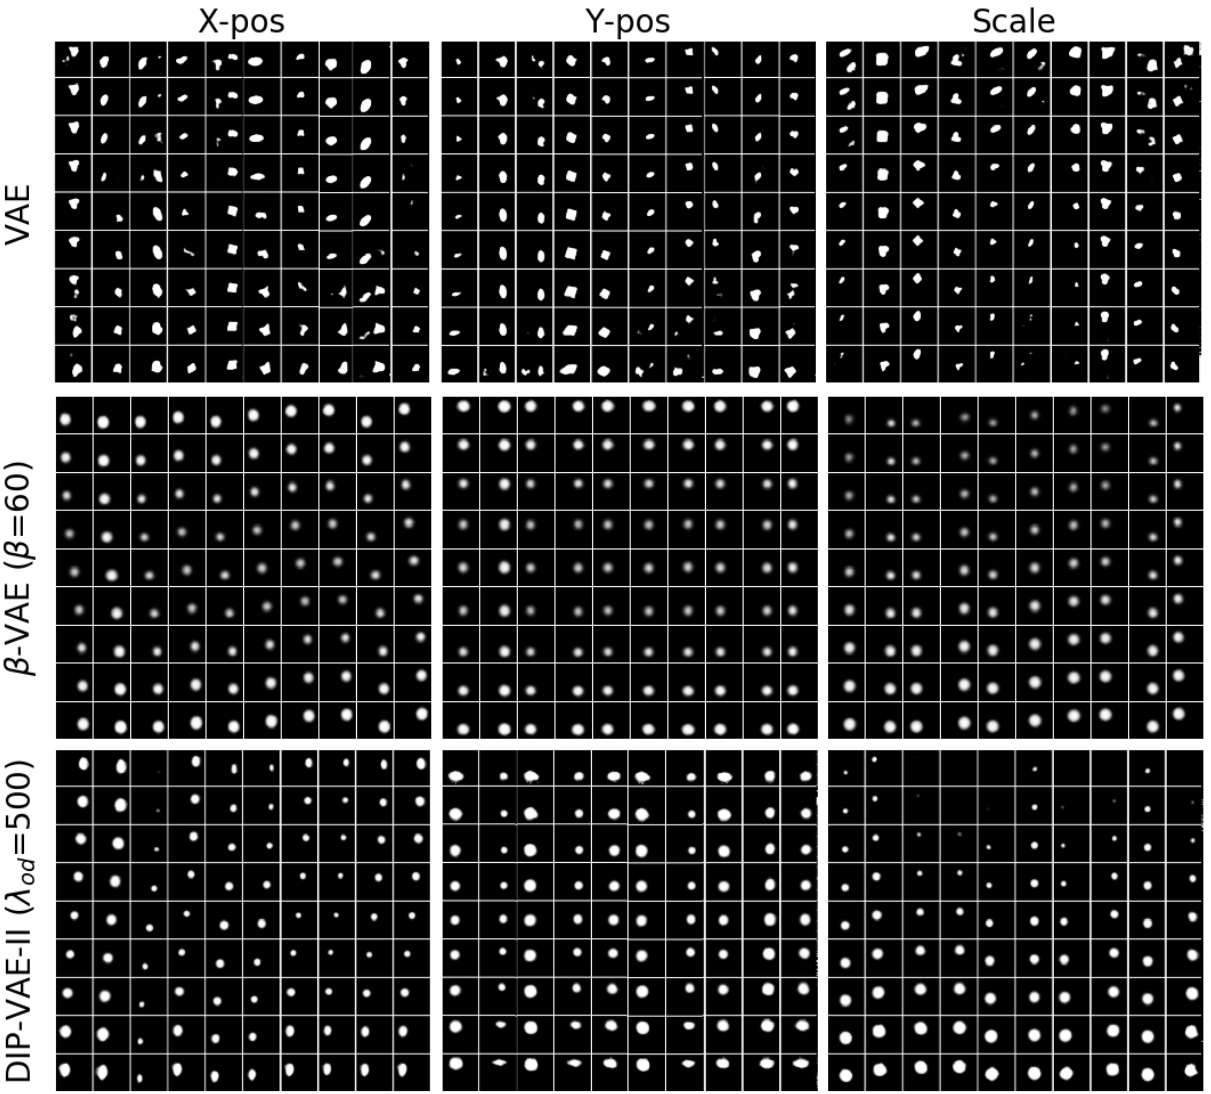
\includegraphics[width=0.75\linewidth]{figs/dip-vae_1}
	\end{figure}

	\myfootnotewithlink{https://arxiv.org/abs/1711.00848}{Kumar A., Sattigeri P., Balakrishnan A. Variational Inference of Disentangled Latent Concepts from Unlabeled Observations, 2017}
\end{frame}
%=======
\begin{frame}{DIP-VAE}
	\begin{figure}
		\centering
		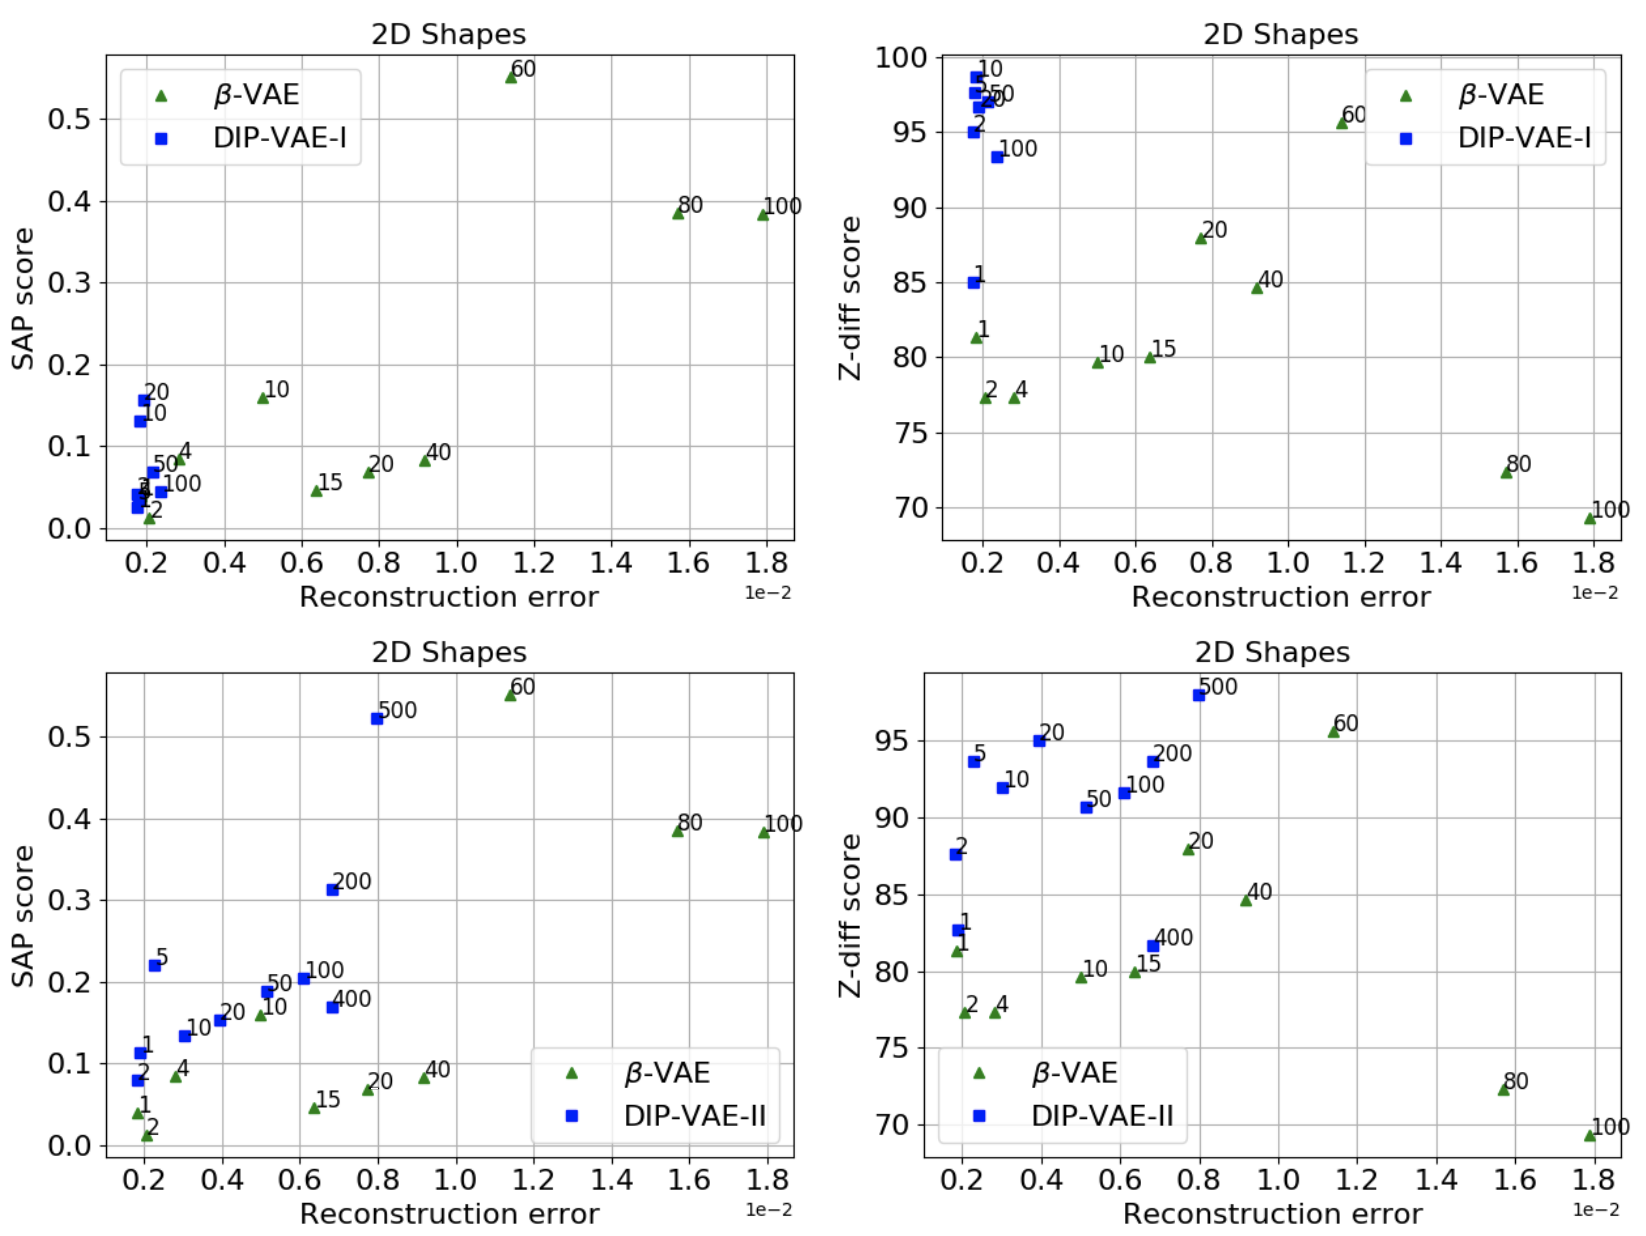
\includegraphics[width=0.9\linewidth]{figs/dip-vae_2}
	\end{figure}

	\myfootnotewithlink{https://arxiv.org/abs/1711.00848}{Kumar A., Sattigeri P., Balakrishnan A. Variational Inference of Disentangled Latent Concepts from Unlabeled Observations, 2017}
\end{frame}
%=======
\begin{frame}{Challenging Disentanglement Assumptions}
Whether unsupervised disentanglement learning is even possible for arbitrary generative models?

\begin{block}{Theorem}
	For $d > 1$, let $\bz \sim P$ denote any distribution which admits a density $p(\bz) = \prod^d_{i=1} p(z_i)$. Then, there exists an infinite family of bijective functions $f : \text{supp}(\bz) \rightarrow \text{supp}(\bz)$ such that
	\begin{itemize}
		\item $\frac{\partial f_i(\bu)}{\partial u_j} \neq 0$ almost everywhere for all $i$ and $j$ (i.e., $\bz$ and $f(\bz)$ are completely entangled);
		\item and $P(\bz \leq \bu) = P(f(\bz) \leq \bu)$ for all $\bu \in \text{supp}(\bz)$ (i.e., they
		have the same marginal distribution).
	\end{itemize}  
\end{block}

Theorem claims that unsupervised disentanglement learning is impossible for arbitrary generative models with a factorized prior.

\myfootnotewithlink{https://arxiv.org/abs/1811.12359}{Locatello F. et al. Challenging Common Assumptions in the Unsupervised Learning of Disentangled Representations, 2018}
\end{frame}
%=======
\begin{frame}{Challenging Disentanglement Assumptions}
Assume we have $p(\bz)$ and some $p(\bx|\bz)$ defining a generative model. Consider any unsupervised
disentanglement method and assume that it finds a representation that is perfectly disentangled with respect
to $\bz$ in the generative model.
\begin{itemize}
	\item Theorem claims that $\exists$ $\hat{\bz} = f(\bz)$ where $\hat{\bz}$ is completely entangled
	with respect to $\bz$.
	\item Since the (unsupervised) disentanglement method only has access to
	observations $\bx$, it hence cannot distinguish between the two equivalent generative models and thus has to be entangled to at least one of them
	\[
	p(\bx) = \int p(\bx | \bz) p(\bz) d\bz = \int p(\bx | \hat{\bz})p(\hat{\bz}) d \hat{\bz}.
	\]
\end{itemize}

\myfootnotewithlink{https://arxiv.org/abs/1811.12359}{Locatello F. et al. Challenging Common Assumptions in the Unsupervised Learning of Disentangled Representations, 2018}
\end{frame}
%=======
\begin{frame}{Challenging Disentanglement Assumptions}
\begin{block}{Proof (1)}
	\begin{enumerate}
		\item 
		Consider the function $g: \text{supp}(\bz) \rightarrow [0, 1]^d$:
		\vspace{-0.1cm}
		\[
		g_i(\bv) = P(z_i \leq v_i), \quad i=1, \dots, d.
		\]
		\vspace{-0.4cm}
		\begin{itemize}
			\item $g$ is bijective (since $p(\bz) = \prod_{i=1}dp(z_i)$).
			\item $\frac{\partial g_i(\bu)}{\partial u_i} \neq 0$, for all $i$ and $\frac{\partial g_i(\bu)}{\partial u_j} = 0$ for all $i \neq j$.
			\item $g(\bz)$ is an independent $d$-dimensional uniform distribution.
		\end{itemize}
		\item 
		Consider $h: (0, 1]^d \rightarrow \bbR^d$
		\[
		h_i(\bv) = \psi^{-1}(v_i), \quad i= 1, \dots, d.
		\]
		Here $\psi$  denotes the CDF of a standard normal distribution.
		\begin{itemize}
			\item $h$ is bijective.
			\item $\frac{\partial g_i(\bu)}{\partial u_i} \neq 0$, for all $i$ and $\frac{\partial g_i(\bu)}{\partial u_j} = 0$ for all $i \neq j$.
			\item $h(g(\bz))$  is a $d$-dimensional standard normal distribution.
		\end{itemize}
	\end{enumerate}
\end{block}

\myfootnotewithlink{https://arxiv.org/abs/1811.12359}{Locatello F. et al. Challenging Common Assumptions in the Unsupervised Learning of Disentangled Representations, 2018}
\end{frame}
\begin{frame}{Challenging Disentanglement Assumptions}
\begin{block}{Proof (2)}
	Let $\bA \in \bbR^{d \times d}$ be an arbitrary orthogonal matrix with $A_{ij} \neq 0$ for all $i, j$.
	The family of such matrices is infinite.
	\begin{itemize}
		\item $\bA$ is orthogonal, it is invertible and thus defines a bijective linear operator. 
		\item $\bA h(g(\bz)) \in \bbR^d$ is hence an independent, multivariate standard normal distribution.
		\item $h^{-1}( \bA h(g(\bz))) \in \bbR^d$ is an independent $d$-dimensional uniform distribution.
	\end{itemize}
	Define $f: \text{supp}(\bz) \rightarrow \text{supp}(\bz)$:
	\[
	f(\bu) = g^{-1} (h^{-1}( \bA h(g(\bz)))).
	\]
	By definition $f(\bz)$ has the same marginal distribution as $\bz$: $P(\bz \leq \bu) = P(f(\bz) \leq \bu)$ and $\frac{\partial f_i(\bu)}{\partial u_j} \neq 0$.
\end{block}

\myfootnotewithlink{https://arxiv.org/abs/1811.12359}{Locatello F. et al. Challenging Common Assumptions in the Unsupervised Learning of Disentangled Representations, 2018}
\end{frame}
%=======
\begin{frame}{Challenging Disentanglement Assumptions}
\begin{itemize}
	\item \textbf{Training:} Factorizing \textbf{samples} from aggregated posterior $q(\bz) = \prod_{i=1}^d q(z_i)$.
	\item \textbf{Inference:} Use a \textbf{mean} vector (usually mean of Gaussian encoder) as a representation.
\end{itemize}
\begin{figure}
	\centering
	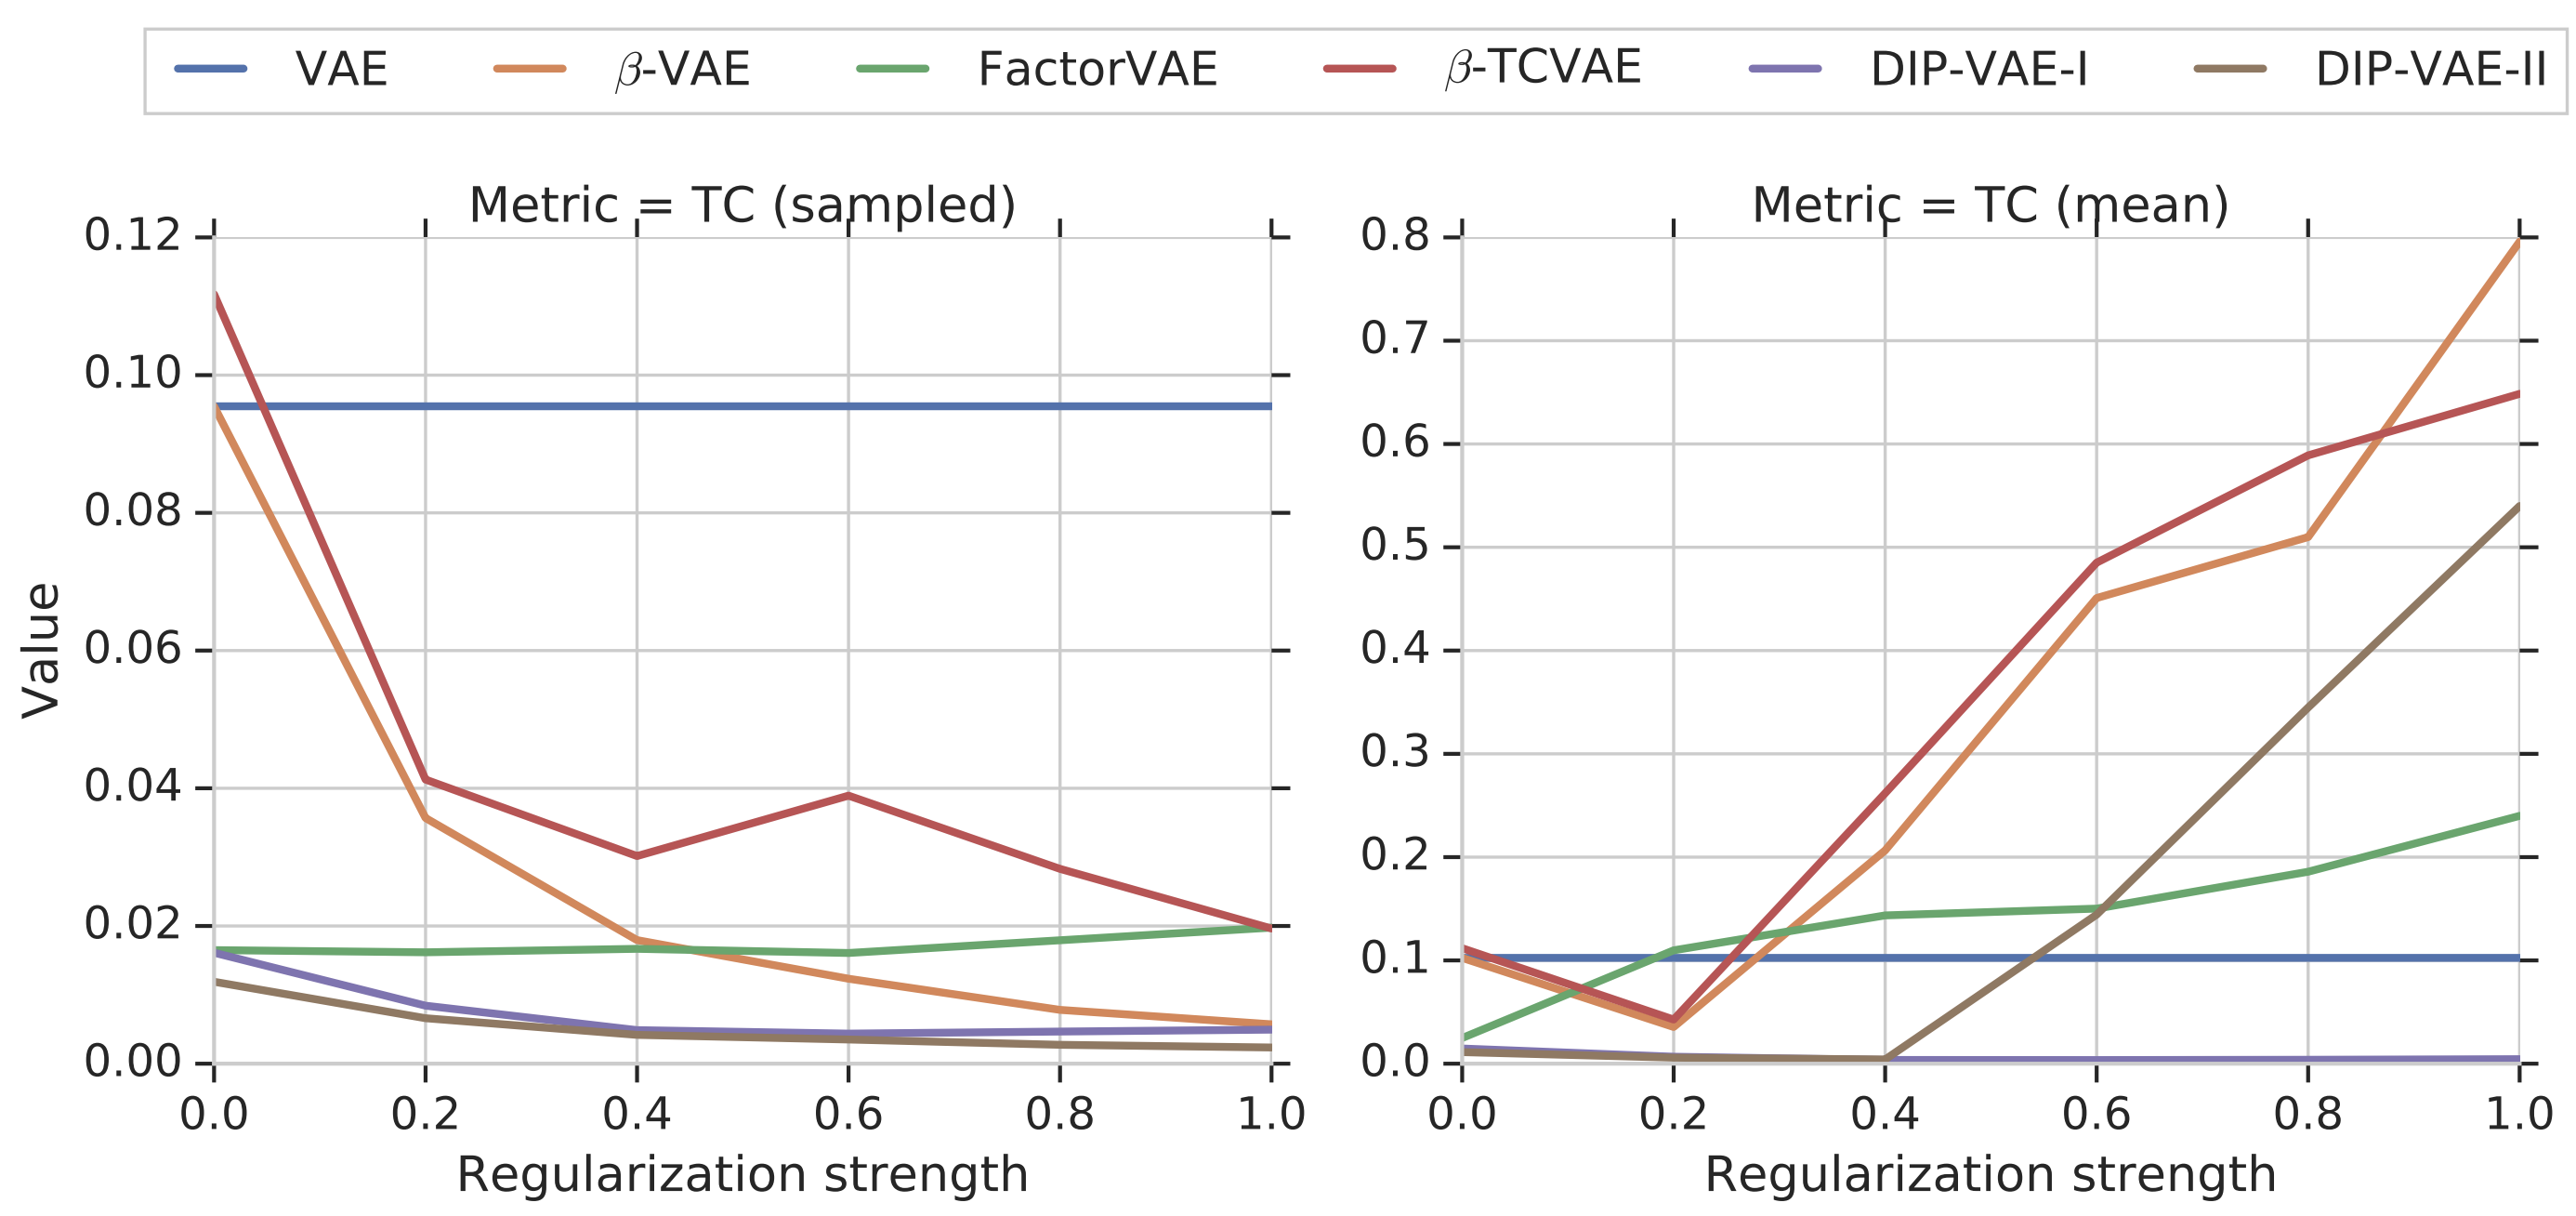
\includegraphics[width=0.95\linewidth]{figs/challenge_dis_1}
\end{figure}

\myfootnotewithlink{https://arxiv.org/abs/1811.12359}{Locatello F. et al. Challenging Common Assumptions in the Unsupervised Learning of Disentangled Representations, 2018}
\end{frame}
%=======
\begin{frame}{Challenging Disentanglement Assumptions}
\begin{block}{Importance of different models and hyperparameters for disentanglement}
	\begin{figure}
		\centering
		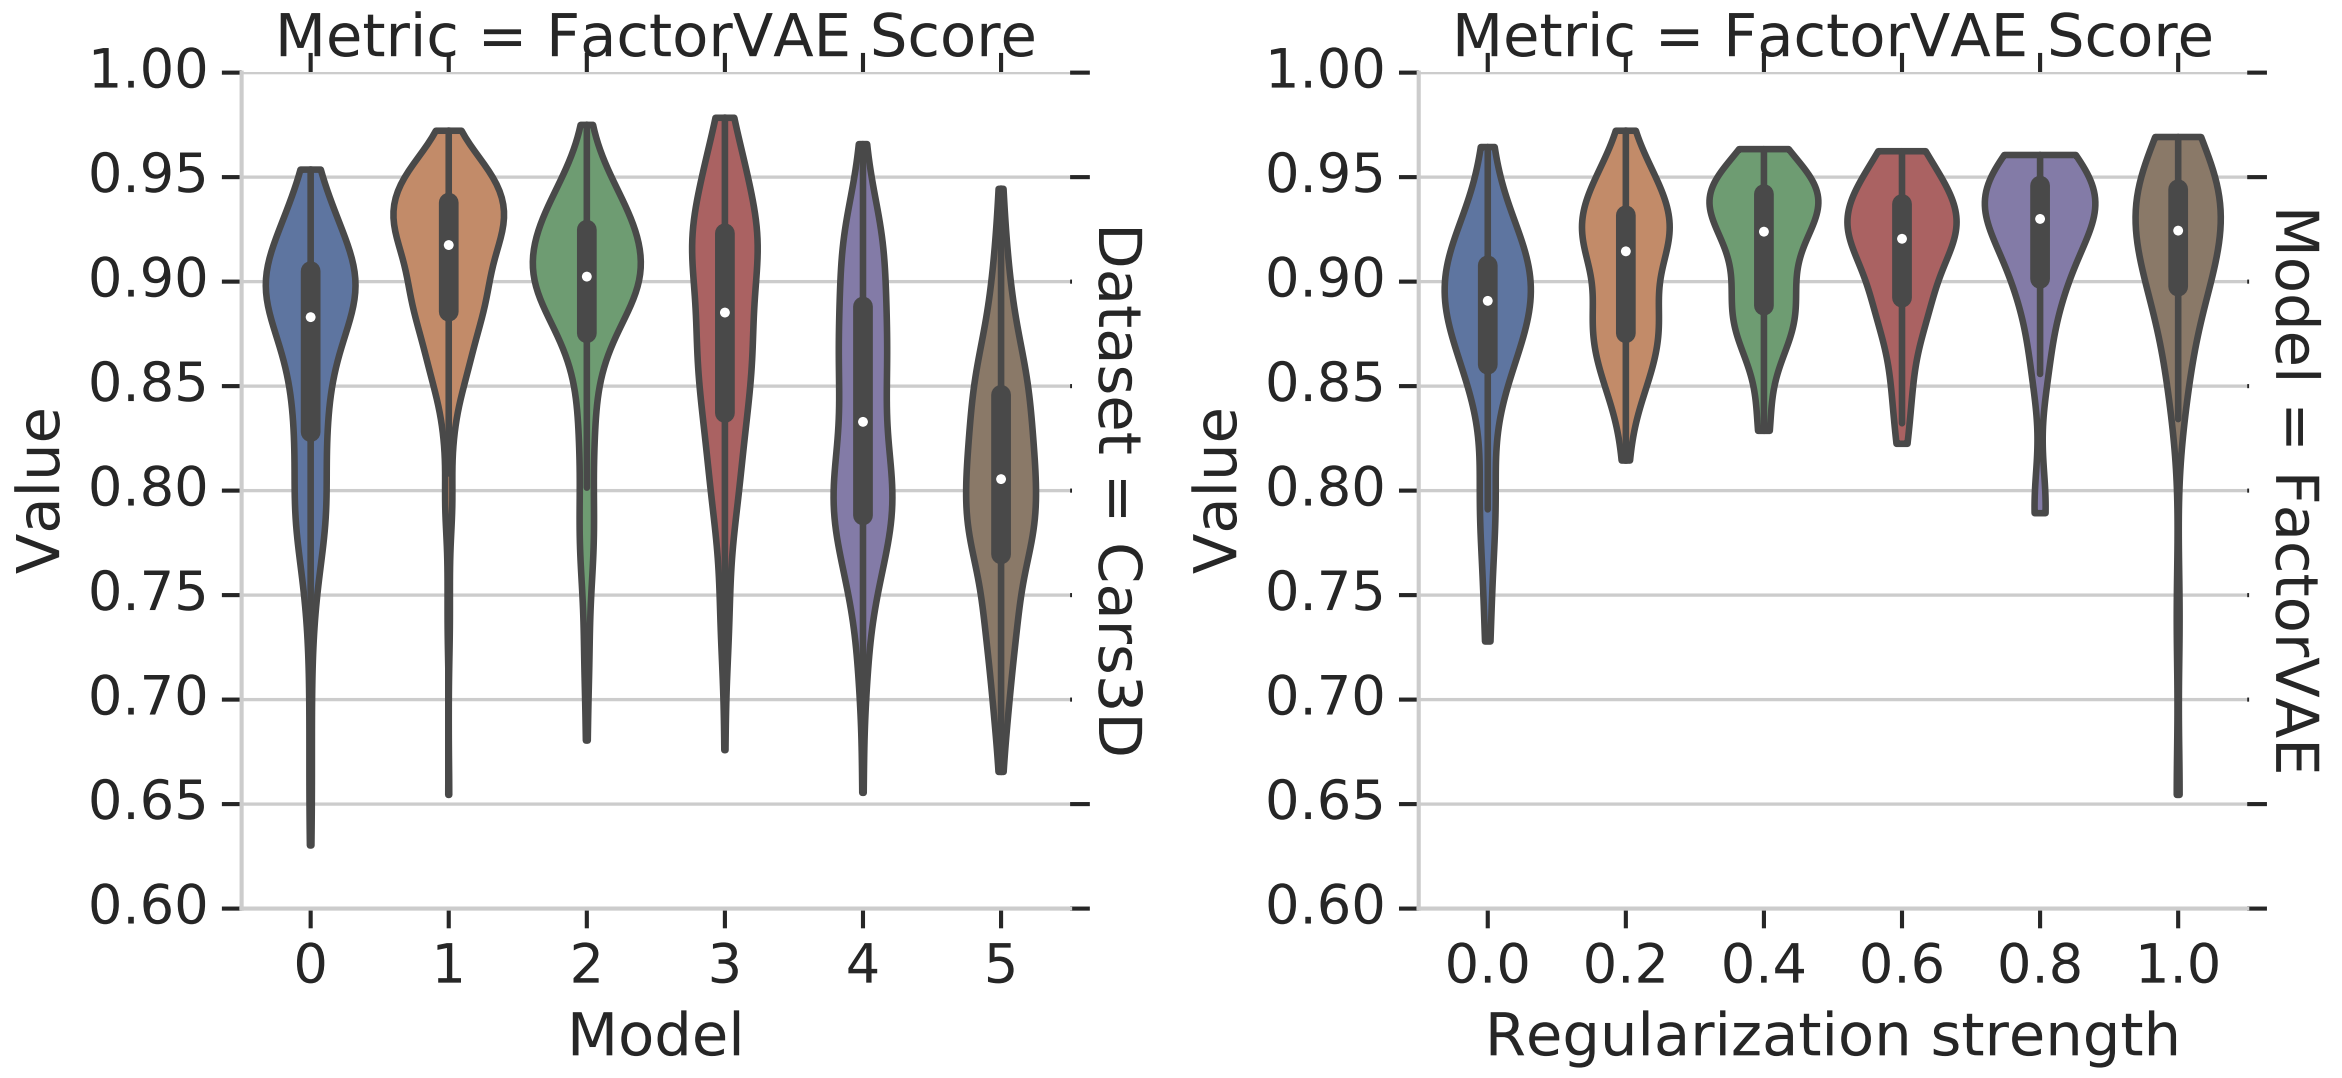
\includegraphics[width=\linewidth]{figs/challenge_dis_2}
	\end{figure}
\end{block}

\myfootnotewithlink{https://arxiv.org/abs/1811.12359}{Locatello F. et al. Challenging Common Assumptions in the Unsupervised Learning of Disentangled Representations, 2018}
\end{frame}
%=======
\begin{frame}{Challenging Disentanglement Assumptions}
\begin{block}{Agreement of different disentanglement metrics}
	\begin{figure}
		\centering
		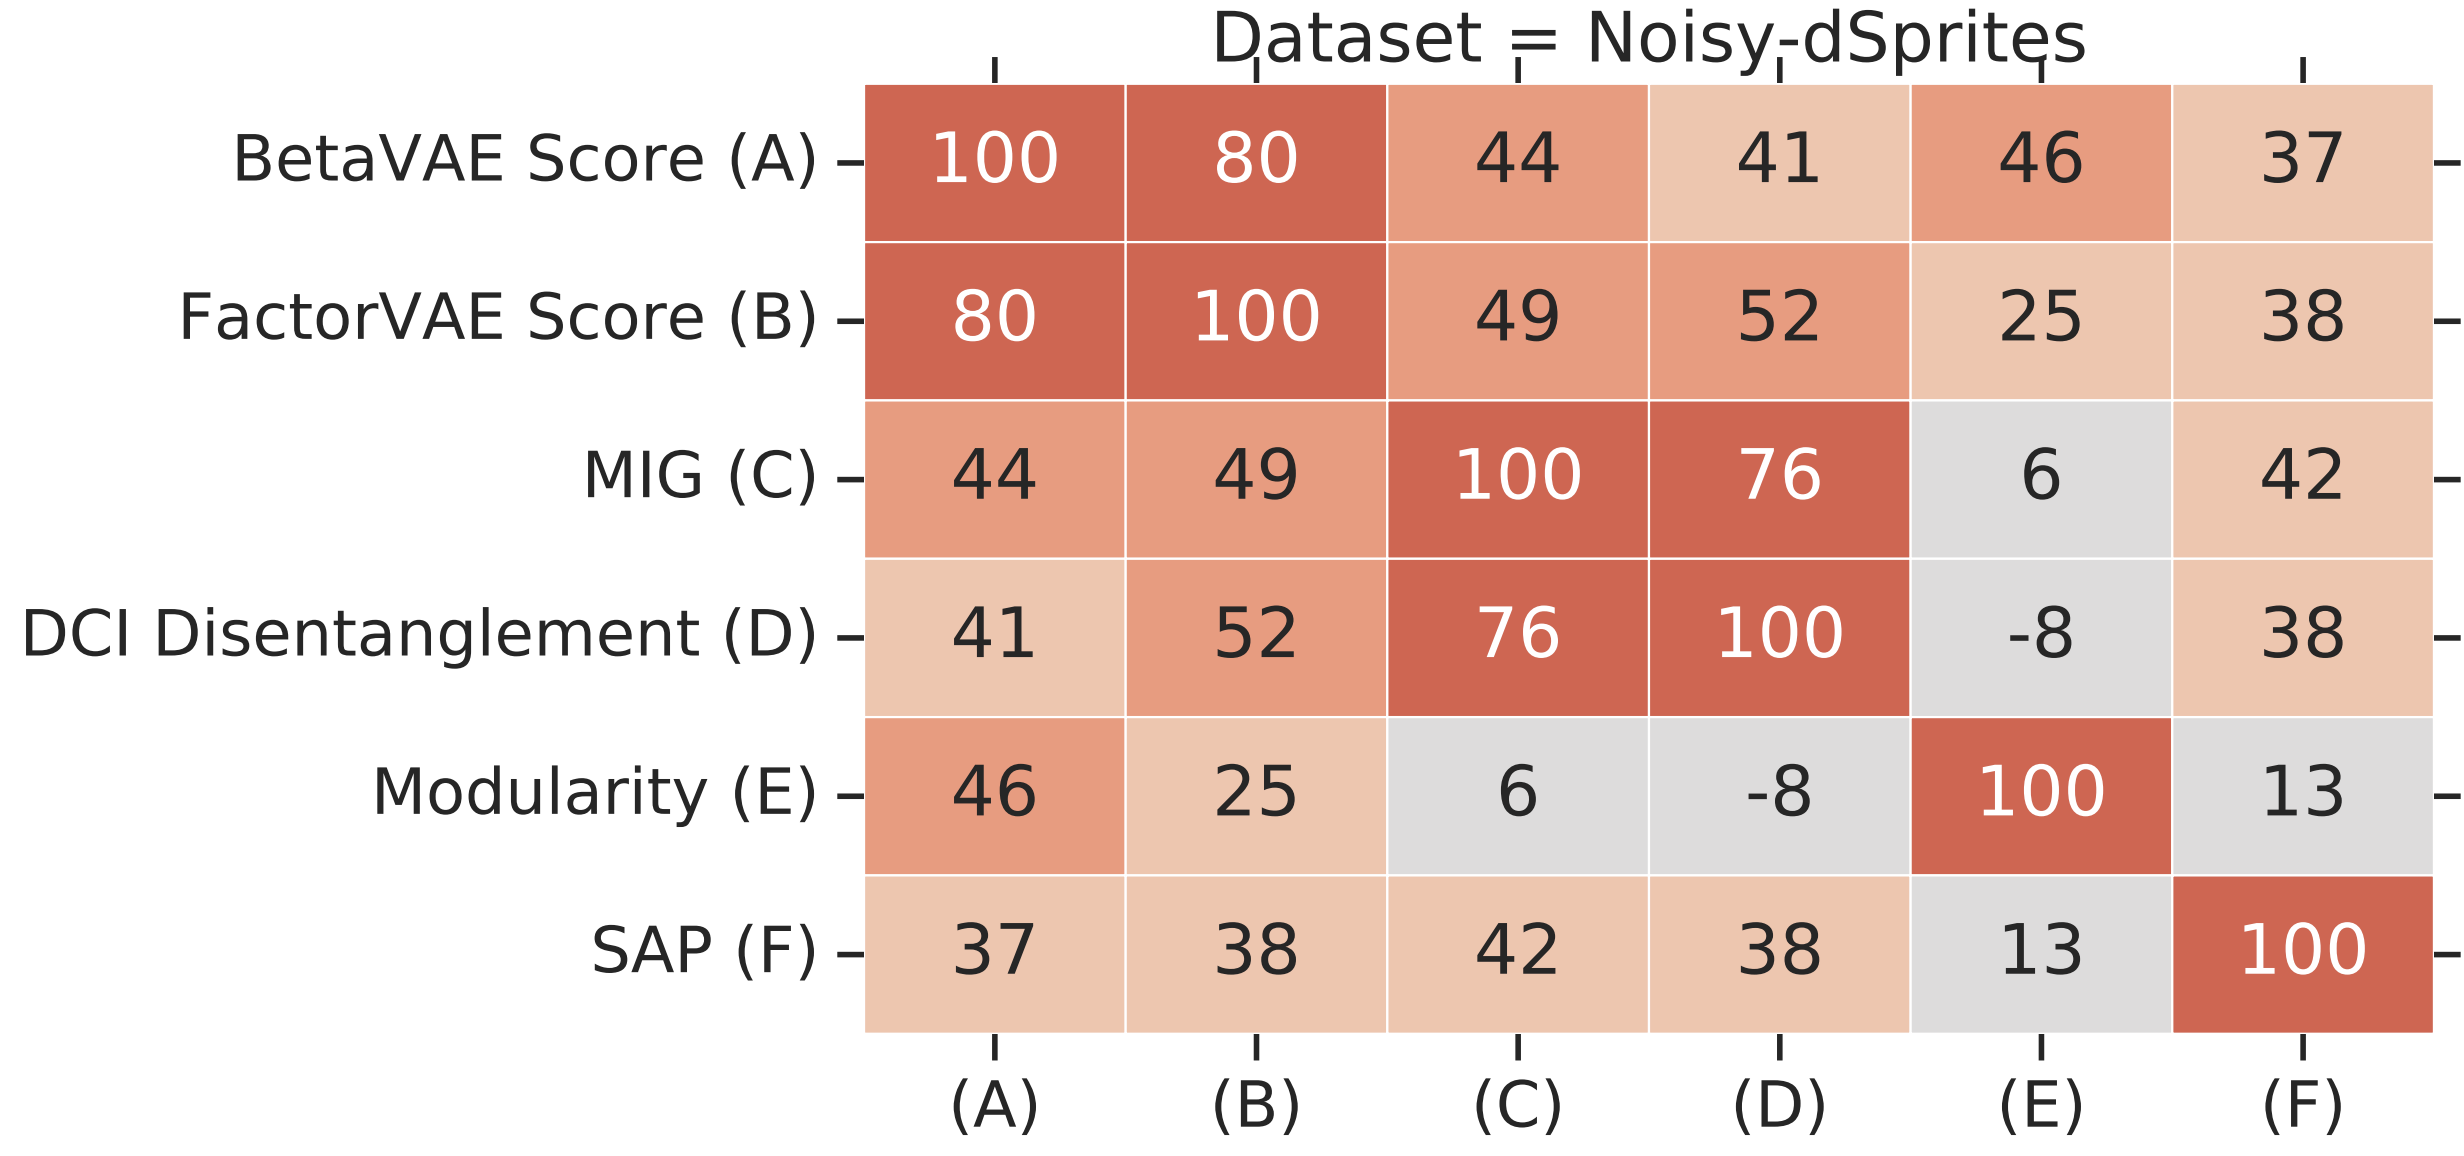
\includegraphics[width=0.9\linewidth]{figs/challenge_dis_3}
	\end{figure}
	\vspace{0.5cm}
\end{block}

\myfootnotewithlink{https://arxiv.org/abs/1811.12359}{Locatello F. et al. Challenging Common Assumptions in the Unsupervised Learning of Disentangled Representations, 2018}
\end{frame}
%=======
\begin{frame}{Generative models zoo}
	\begin{figure}
		\centering
		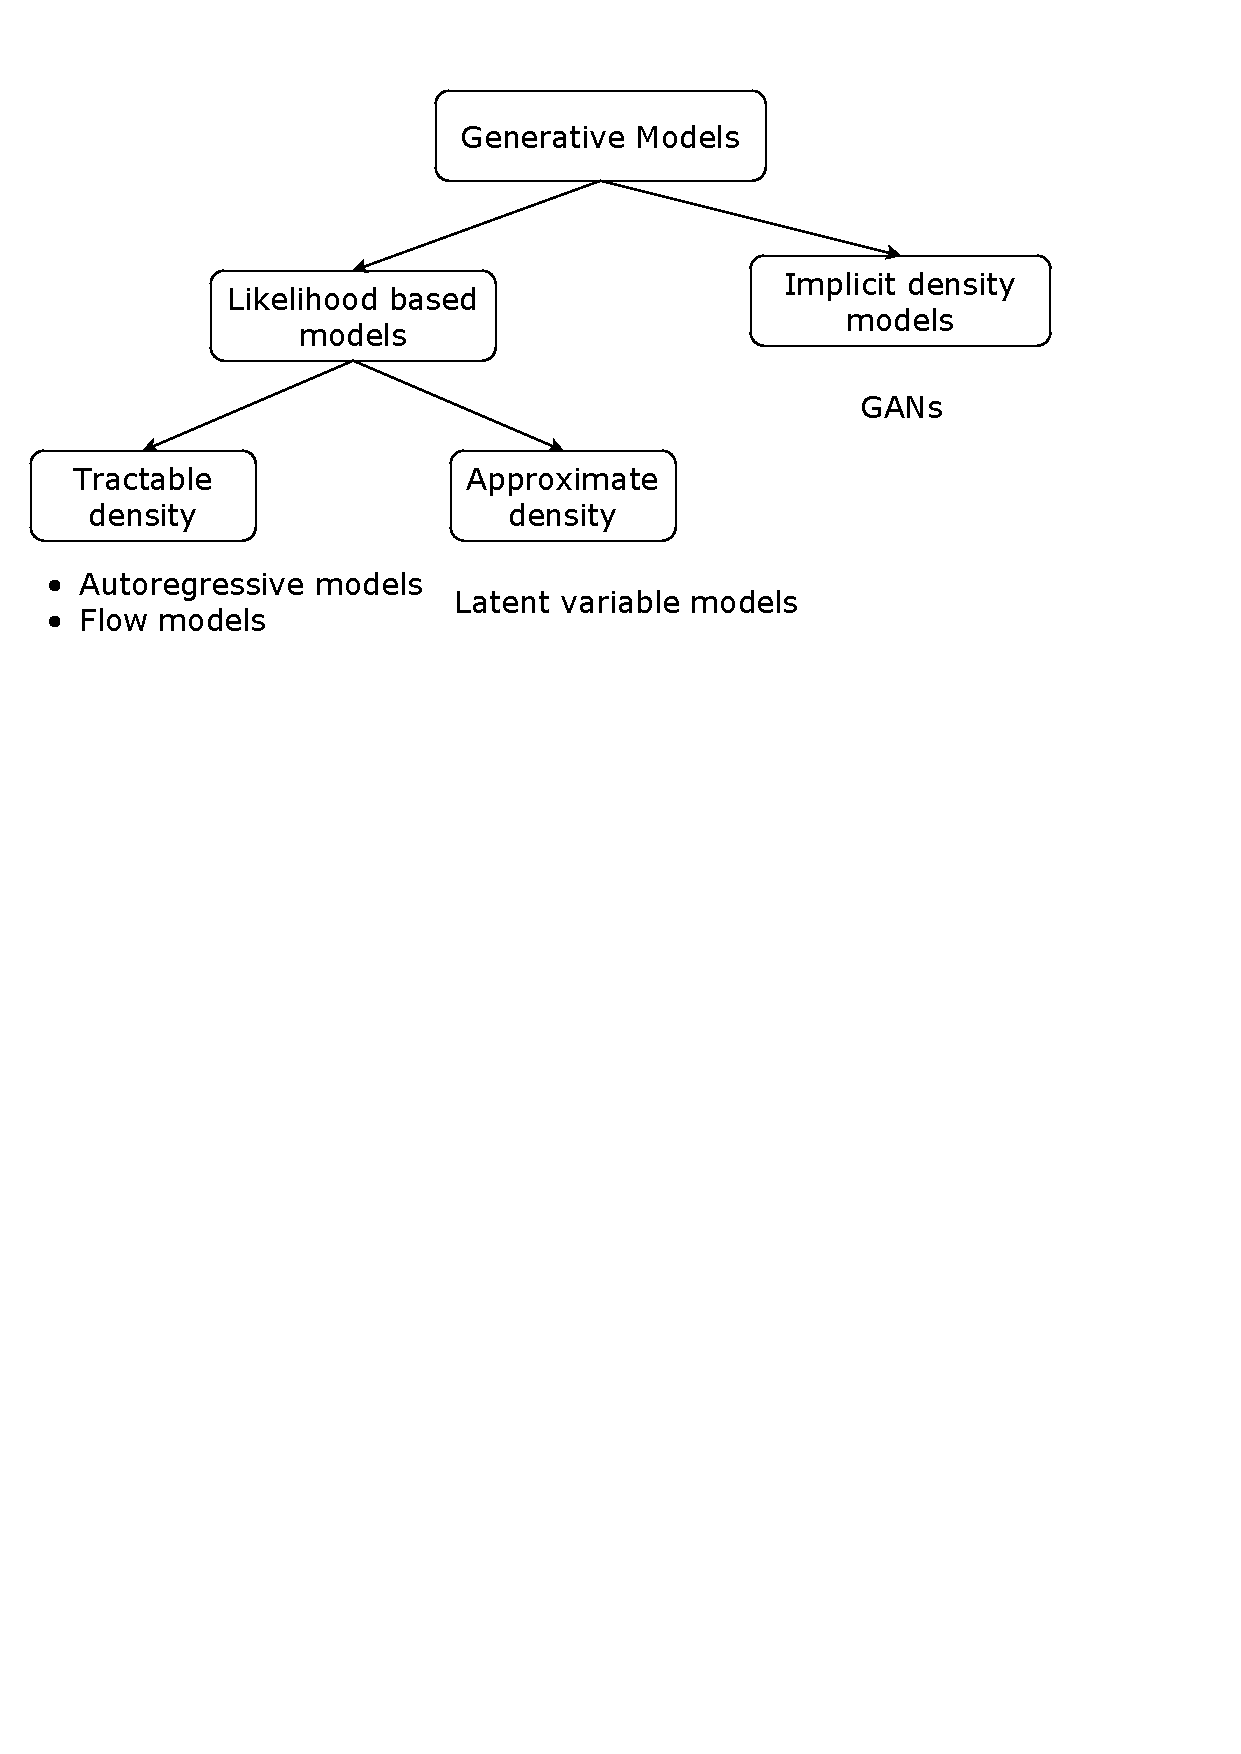
\includegraphics[width=1.0\linewidth]{figs/generative_models_zoo.pdf}
	\end{figure}
\end{frame}
%=======
\begin{frame}{Likelihood based models}
	Is likelihood a good measure of model quality?
	\begin{minipage}[t]{0.48\columnwidth}
		\begin{block}{Poor likelihood \\ Great samples}
			\vspace{-0.3cm}
			\[
				p_1(\bx) = \frac{1}{n} \sum_{i=1}^n \cN(\bx | \bx_i, \epsilon \bI)
			\]
			For small $\epsilon$ this model will generate samples with great quality, but likelihood will be very poor.
		\end{block}
	\end{minipage}%
	\begin{minipage}[t]{0.52\columnwidth}
		\begin{block}{Great likelihood \\ Poor samples}
			\vspace{-0.3cm}
			\[
				p_2(\bx) = 0.01p(\bx) + 0.99p_{\text{noise}}(\bx)
			\]
			\begin{multline*}
				\log \left[ 0.01p(\bx) + 0.99p_{\text{noise}}(\bx) \right] \geq  \\ \geq \log \left[ 0.01p(\bx) \right]  = \log p(\bx) - \log 100
			\end{multline*}
		Noisy irrelevant samples, but for high dimensions $\log p(\bx)$ becames larger.
		\end{block}
	\end{minipage}
	\myfootnotewithlink{https://arxiv.org/abs/1511.01844}{Theis L., Oord A., Bethge M. A note on the evaluation of generative models, 2015}
\end{frame}
%=======
\begin{frame}{Likelihood-free learning}
	\begin{itemize}
		\item Likelihood is not a perfect measure for quality measure for generative model.
		\item Likelihood could be intractable.
	\end{itemize}
	\begin{block}{Where did we start}
	 We would like to approximate true data distribution $\pi(\bx)$.
		Instead of searching true $\pi(\bx)$ over all probability distributions, learn function approximation $p(\bx | \btheta) \approx \pi(\bx)$.
	\end{block}
	Imagine we have two sets of samples 
	\begin{itemize}
		\item $\cS_1 = \{\bx_i\}_{i=1}^{n_1} \sim \pi(\bx)$
		\item $\cS_2 = \{\bx_i\}_{i=1}^{n_2} \sim p(\bx | \btheta)$
	\end{itemize}
	\begin{block}{Two sample test}
		\vspace{-0.3cm}
		\[
			H_0: \pi(\bx) = p(\bx | \btheta), \quad H_1: \pi(\bx) \neq p(\bx | \btheta)
		\]
	\end{block}
\end{frame}
%=======
\begin{frame}{Likelihood-free learning}
		\begin{block}{Two sample test}
			\vspace{-0.3cm}
			\[
				H_0: \pi(\bx) = p(\bx | \btheta), \quad H_1: \pi(\bx) \neq p(\bx | \btheta)
			\]
	\end{block}
	Define test statistic $T(\cS_1, \cS_2)$. The test statictic is likelihood free.
	
	If $T(\cS_1, \cS_2) < \alpha$, then accept $H_0$, else reject it.
	
	\begin{block}{Desired behaviour}
		\begin{itemize}
			\item The generative model $p(\bx | \btheta)$ minimizes the value of test statistic~$T(\cS_1, \cS_2)$.
			\item It is hard to find an appropriate test statistic in high dimensions. We could try to learn the appropriate $T(\cS_1, \cS_2)$.
		\end{itemize}
	\end{block}
\end{frame}
%=======
\begin{frame}{Vanila GAN}
	\begin{itemize}
		\item \textbf{Generator:} latent variable model $\bx = G(\bz)$, which minimizes two-sample test objective.
		\item \textbf{Discriminator:} function $D(\bx)$, which distinguishes real samples from model samples and maximizes a two-sample test statistic.
	\end{itemize}
	\begin{block}{Objective}
		\[
			V(G, D) = \min_{G} \max_D \bbE_{\pi(\bx)} \log D(\bx) + \bbE_{p(\bz)} \log (1 - D(G(\bz)))
		\]
	\end{block}
	For fixed generator $G(\bz)$ the discriminator is performing a binary classification with a cross entropy loss.
	
	 This minimax game has the global optimum $\pi(\bx) = p(\bx | \btheta)$.
	 \myfootnotewithlink{https://arxiv.org/abs/1406.2661}{Goodfellow I. J. et al. Generative Adversarial Networks, 2014}
\end{frame}
%=======
\begin{frame}{Vanila GAN optimality}
	
	\begin{block}{Objective (fixed $G$)}
		\[
		\max_D V(D) = \bbE_{\pi(\bx)} \log D(\bx) + \bbE_{p(\bz)} \log (1 - D(G(\bz)))
		\]
	\end{block}
	\begin{block}{Optimal discriminator}
		\vspace{-0.5cm}
		\begin{align*}
			V(G, D) &= \bbE_{\pi(\bx)} \log D(\bx) + \bbE_{p(\bx | \btheta)} \log (1 - D(\bx)) \\
			&= \int \underbrace{\left[ \pi(\bx) \log D(\bx) + p(\bx | \btheta)\log (1 - D(\bx) \right]}_{y(D)} d \bx
		\end{align*}
		\[
			\frac{d y(D)}{d D} = \frac{\pi(\bx)}{D(\bx)} - \frac{p(\bx | \btheta)}{1 - D(\bx)} = 0 \quad \Rightarrow \quad D^*(\bx) = \frac{\pi(\bx)}{\pi(\bx) + p(\bx | \btheta)}
		\]
	\end{block}
	\myfootnotewithlink{https://arxiv.org/abs/1406.2661}{Goodfellow I. J. et al. Generative Adversarial Networks, 2014}

\end{frame}
%=======
\begin{frame}{Vanila GAN optimality}
	
	\begin{block}{Objective (fixed $D$)}
		\[
		\max_G V(G, D^*) = \bbE_{\pi(\bx)} \log D^*(\bx) + \bbE_{p(\bz)} \log (1 - D^*(G(\bz)))
		\]
	\end{block}
	\begin{block}{Optimal generator}
		\vspace{-0.5cm}
		\begin{multline*}
			V(G, D^*) = \bbE_{\pi(\bx)} \log \frac{\pi(\bx)}{\pi(\bx) + p(\bx | \btheta)} + \bbE_{p(\bx | \btheta)} \log \frac{p(\bx | \btheta)}{\pi(\bx) + p(\bx | \btheta)} \\
			 = KL \left(\pi(\bx) || \frac{\pi(\bx) + p(\bx | \btheta)}{2}\right) + KL \left(p(\bx | \btheta) || \frac{\pi(\bx) + p(\bx | \btheta)}{2}\right) - 2\log 2 \\
			 = 2JSD(\pi(\bx) || p(\bx | \btheta)) - 2\log 2.
		\end{multline*}
	\end{block}
	 \myfootnotewithlink{https://arxiv.org/abs/1406.2661}{Goodfellow I. J. et al. Generative Adversarial Networks, 2014}
\end{frame}
%=======
\begin{frame}{Vanila GAN optimality}
	\begin{block}{Optimal generator}
		\vspace{-0.2cm}
		\[
			V(G, D^*)  = 2JSD(\pi(\bx) || p(\bx | \btheta)) - 2\log 2.
		\]
	\end{block}
	\begin{block}{Jensen-Shannon divergence}
		\vspace{-0.2cm}
		\footnotesize
		\[
			JSD(\pi(\bx) || p(\bx | \btheta)) = \frac{1}{2} \left[KL \left(\pi(\bx) || \frac{\pi(\bx) + p(\bx | \btheta)}{2}\right) + KL \left(p(\bx | \btheta) || \frac{\pi(\bx) + p(\bx | \btheta)}{2}\right) \right]
		\]
	\end{block}
	Also called symmetric KL divergence. Could be used as a distance measure!
	
	\[
		V(G^*, D^*) = -2\log 2, \quad \pi(\bx) = p(\bx | \btheta).
	\]
	If the generator updates are made in a function space and the discriminator is optimal at every step, then the generator is guaranteed to converge to the data distribution.
\end{frame}
%=======
\begin{frame}{Vanila GAN}
	\begin{block}{Objective}
		\vspace{-0.4cm}
		\[
		V(G, D) = \min_{G} \max_D \bbE_{\pi(\bx)} \log D(\bx) + \bbE_{p(\bz)} \log (1 - D(G(\bz)))
		\]
		\vspace{-0.4cm}
	\end{block}

	\begin{figure}
		\centering
		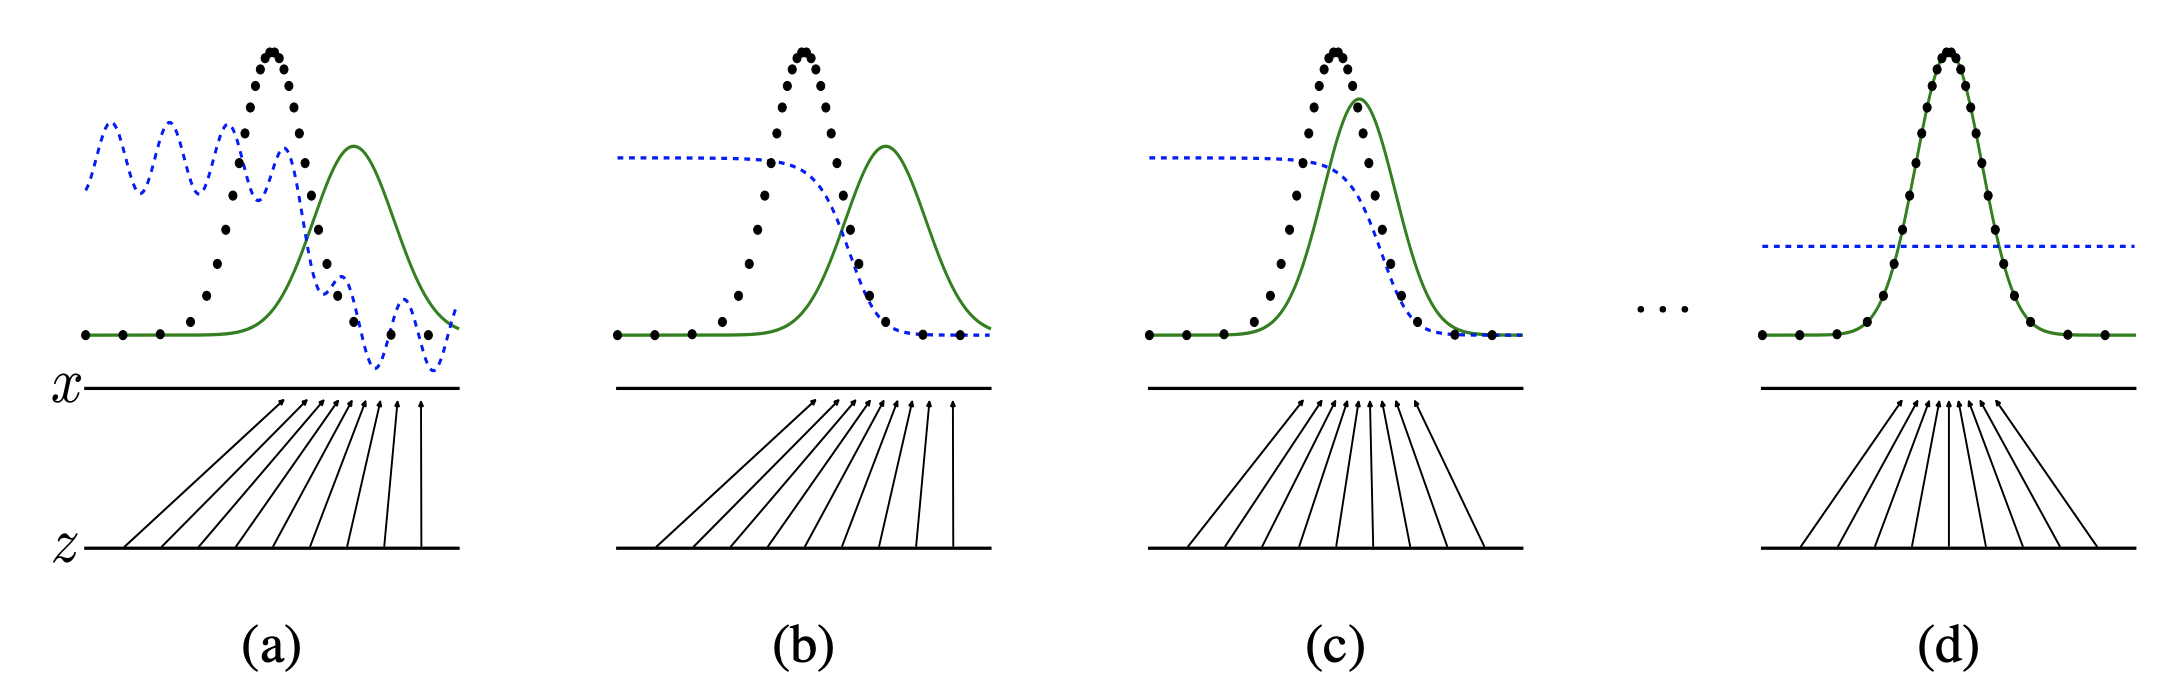
\includegraphics[width=1.0\linewidth]{figs/gan_1}
	\end{figure}
	\begin{itemize}
		\item Generator updates are made in parameter space.
		\item Discriminator is not optimal at every step.
		\item Generator and discriminator loss keeps oscillating during GAN training.
	\end{itemize}

	 \myfootnotewithlink{https://arxiv.org/abs/1406.2661}{Goodfellow I. J. et al. Generative Adversarial Networks, 2014}
\end{frame}
%=======
\begin{frame}{Vanishing gradients}
	\begin{block}{Objective}
		\vspace{-0.4cm}
		\[
		V(G, D) = \min_{G} \max_D \bbE_{\pi(\bx)} \log D(\bx) + \bbE_{p(\bz)} \log (1 - D(G(\bz)))
		\]
		\vspace{-0.4cm}
	\end{block}
	Early in learning, $G$ is poor, $D$ can reject samples with high confidence. In this case, $\log (1 - D(G(\bz)))$ saturates.
	\begin{minipage}[t]{0.5\columnwidth}
		\begin{figure}
			\centering
			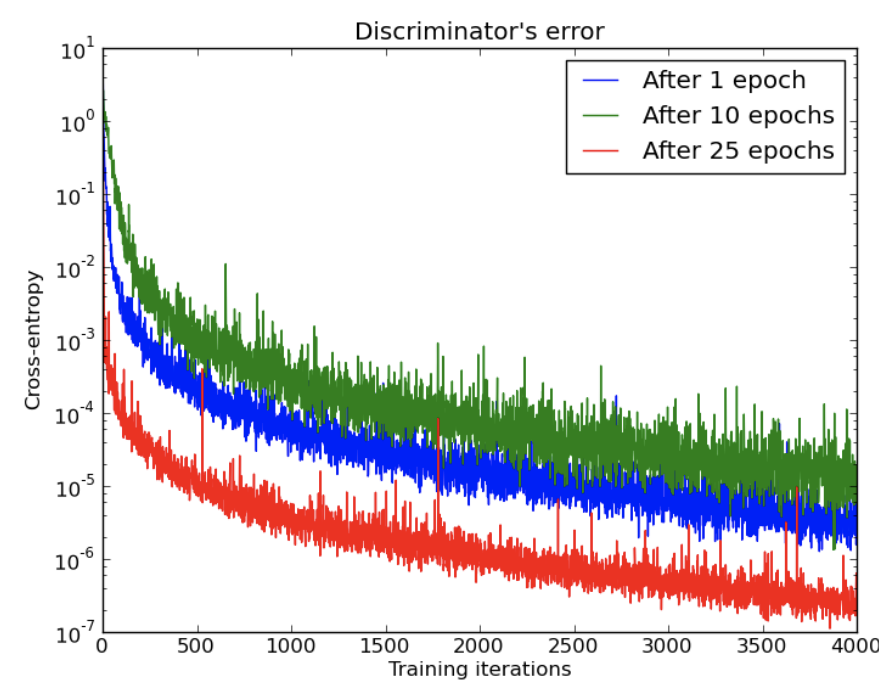
\includegraphics[width=0.9\linewidth]{figs/vanishing_gradients_1}
		\end{figure}
	\end{minipage}%
	\begin{minipage}[t]{0.5\columnwidth}
		\begin{figure}
			\centering
			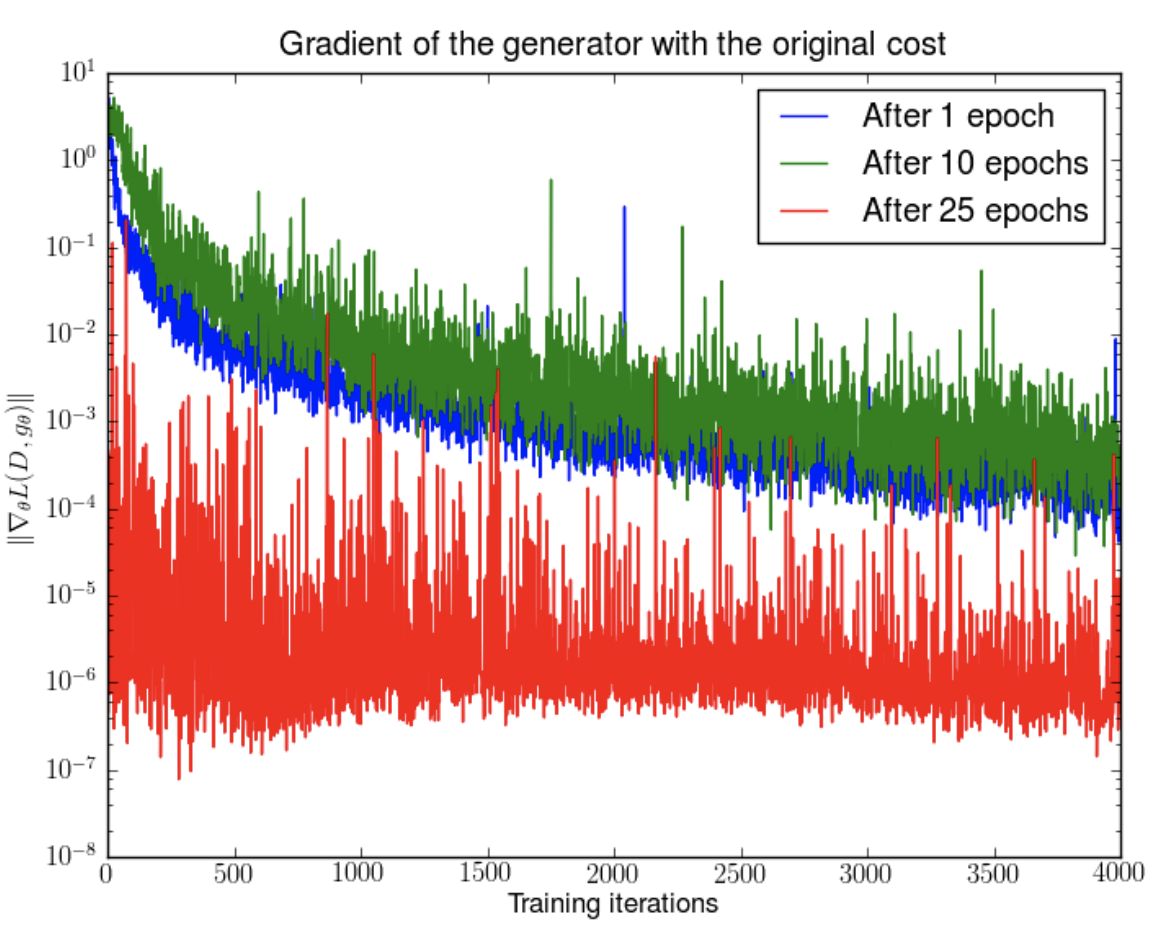
\includegraphics[width=0.9\linewidth]{figs/vanishing_gradients_2}
		\end{figure}
	\end{minipage}
	\myfootnotewithlink{https://arxiv.org/abs/1701.04862}{Arjovsky M., Bottou L. Towards Principled Methods for Training Generative Adversarial Networks, 2017}
\end{frame}
%=======
\begin{frame}{Vanishing gradients}
	\begin{block}{Objective}
		\vspace{-0.4cm}
		\[
		V(G, D) = \min_{G} \max_D \bbE_{\pi(\bx)} \log D(\bx) + \bbE_{p(\bz)} \log (1 - D(G(\bz)))
		\]
		\vspace{-0.4cm}
	\end{block}
	\begin{minipage}[t]{0.45\columnwidth}
		\vspace{0.4cm}
		Maximize $\log D(G(z))$ instead of $\log (1 - D(G(\bz)))$. \\
		Gradients are getting much stronger, but the training is instable (with increasing mean and variance).
	\end{minipage}%
	\begin{minipage}[t]{0.55\columnwidth}
		\begin{figure}
			\centering
			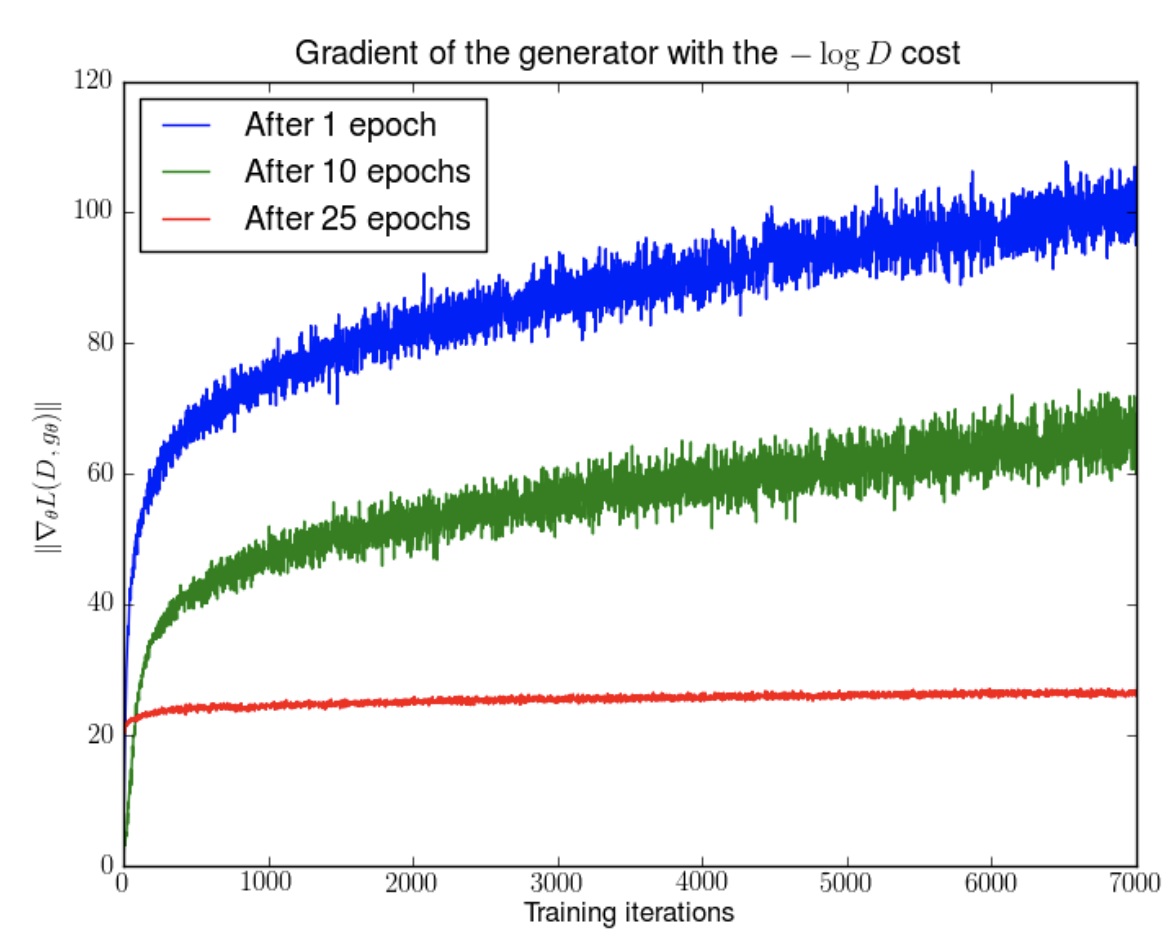
\includegraphics[width=1.0\linewidth]{figs/vanishing_gradients_3}
		\end{figure}
	\end{minipage}
	\myfootnotewithlink{https://arxiv.org/abs/1701.04862}{Arjovsky M., Bottou L. Towards Principled Methods for Training Generative Adversarial Networks, 2017}
\end{frame}
%=======
\begin{frame}{Likelihood-based vs GAN}
	\begin{block}{GAN objective (for optimal discriminator)}
		\vspace{-0.2cm}
		\[
			V(G, D^*)  = 2JSD(\pi(\bx) || p(\bx | \btheta)) - \log 4.
		\]
	\end{block}
	\begin{block}{Likelihood model objective}
		\vspace{-0.6cm}
		\begin{multline*}
			\max_{\btheta} \log p(\bX | \btheta) \approx \max_{\btheta}\bbE_{\pi(\bx)} \log p(\bx | \btheta) = \\ = \max_{\btheta}\bbE_{\pi(\bx)} \log p(\bx | \btheta) - \bbE_{\pi(\bx)} \log \pi(\bx) = \\ = \max_{\btheta}\bbE_{\pi(\bx)}  \log \frac{p(\bx | \btheta)}{\pi(\bx)}= \min_{\btheta} KL(\pi(\bx) || p(\bx | \btheta))
		\end{multline*}
	\vspace{-0.6cm}
	\end{block}

	What is the difference between $JS$ and $KL$ divergences?
\end{frame}
%=======
\begin{frame}{Mode collapse}
	The phenomena where the generator of a GAN collapses to one or few distribution modes.
	\begin{figure}
		\centering
		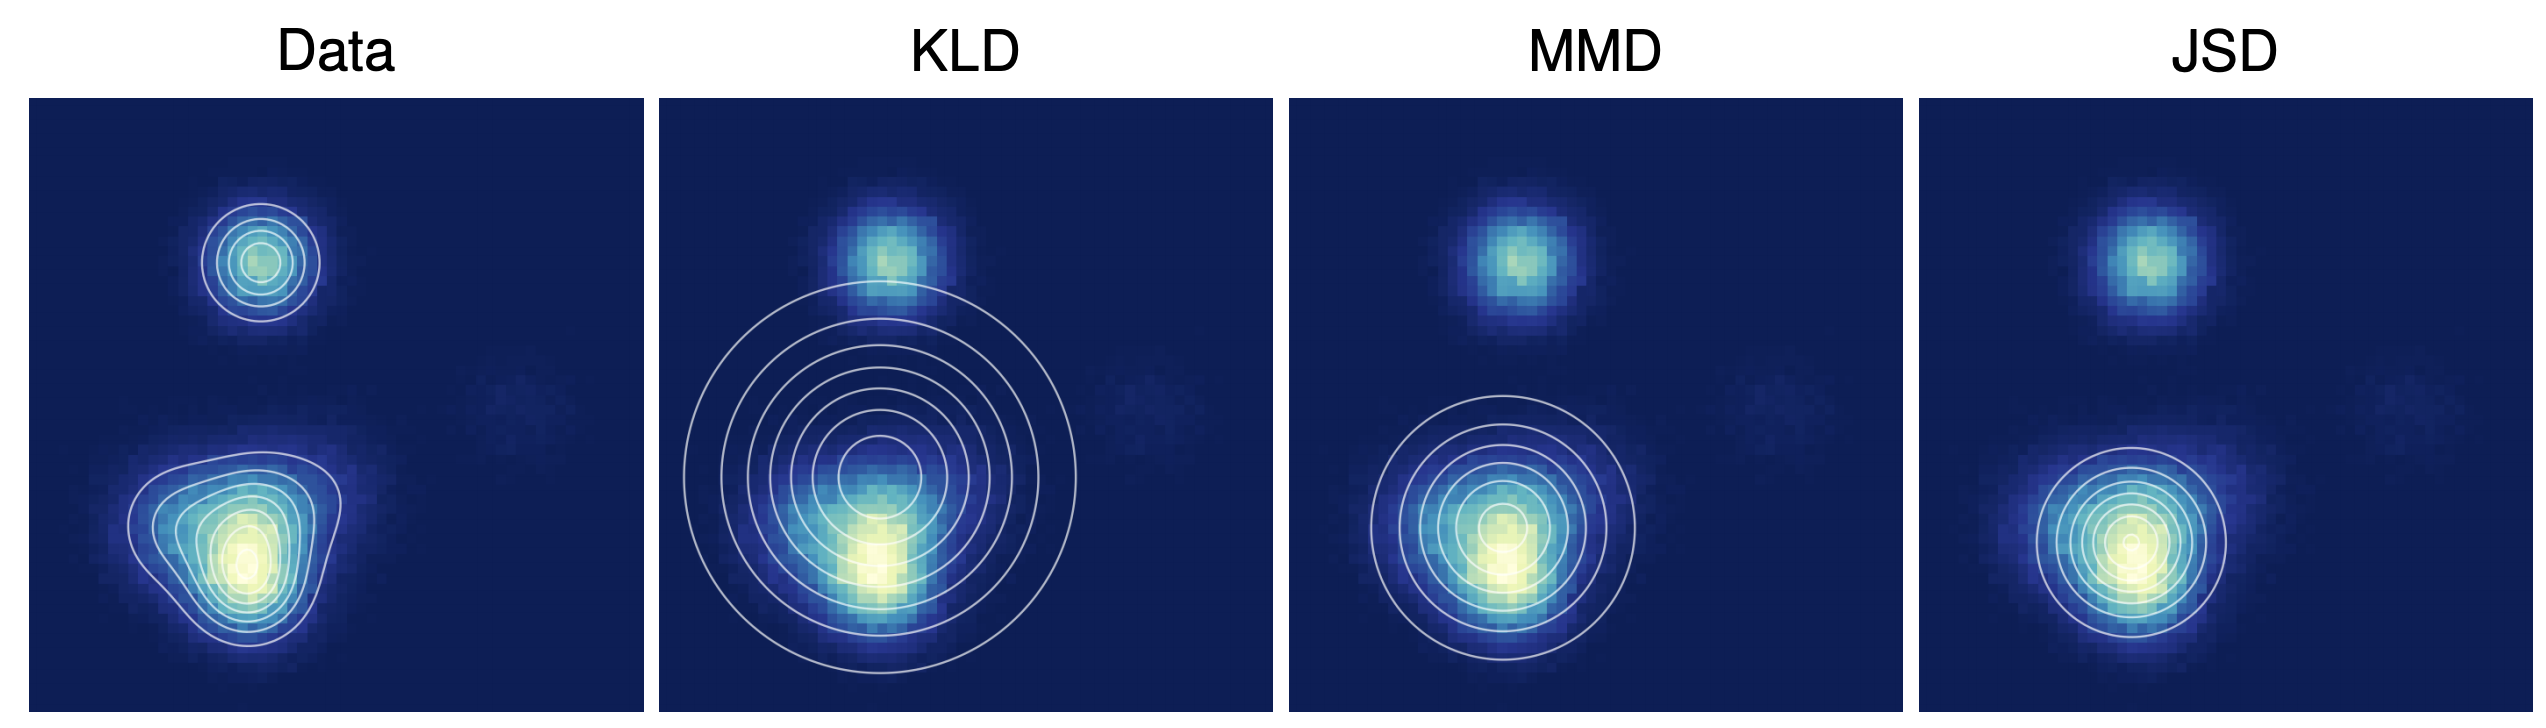
\includegraphics[width=0.9\linewidth]{figs/mode_collapse_1}
	\end{figure}
	\begin{figure}
		\centering
		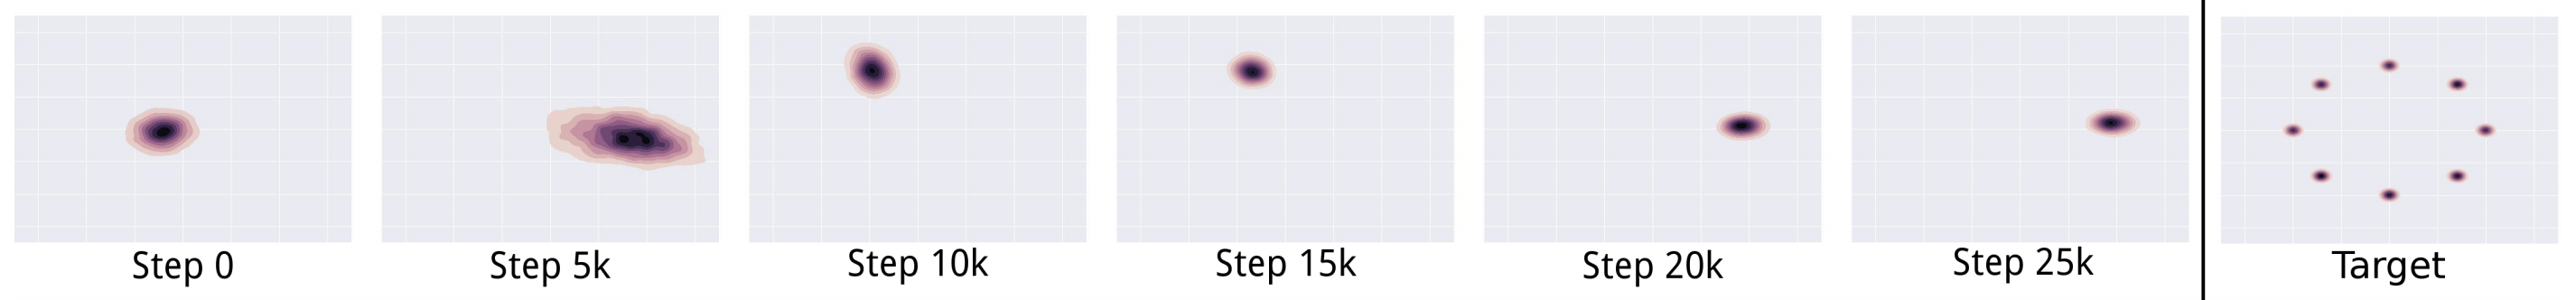
\includegraphics[width=1.0\linewidth]{figs/mode_collapse_3}
	\end{figure}
	Alternate architectures, adding regularization terms, injecting small noise
	perturbations and other millions bags and tricks are used to avoid the mode collapse.
	
	\myfootnote{\href{https://arxiv.org/abs/1406.2661}{Goodfellow I. J. et al. Generative Adversarial Networks, 2014} \\
	\href{https://arxiv.org/abs/1611.02163}{Metz L. et al. Unrolled Generative Adversarial Networks, 2016}}
\end{frame}
%=======
\begin{frame}{Mode collapse}
	\begin{block}{Mode covering vs mode seeking}
		\vspace{-0.2cm}
		\[
			KL(\pi || p) = \int \pi(\bx) \log \frac{\pi(\bx)}{p(\bx)}d\bx, \quad KL(p || \pi) = \int p(\bx) \log \frac{p(\bx)}{\pi(\bx)}d\bx
		\]
		\[
		JSD(\pi || p) = \frac{1}{2} \left[KL \left(\pi(x) || \frac{\pi(\bx) + p(\bx)}{2}\right) + KL \left(p(x) || \frac{\pi(\bx) + p(\bx)}{2}\right) \right]
		\]
		\vspace{-0.4cm}
		\begin{figure}
			\centering
			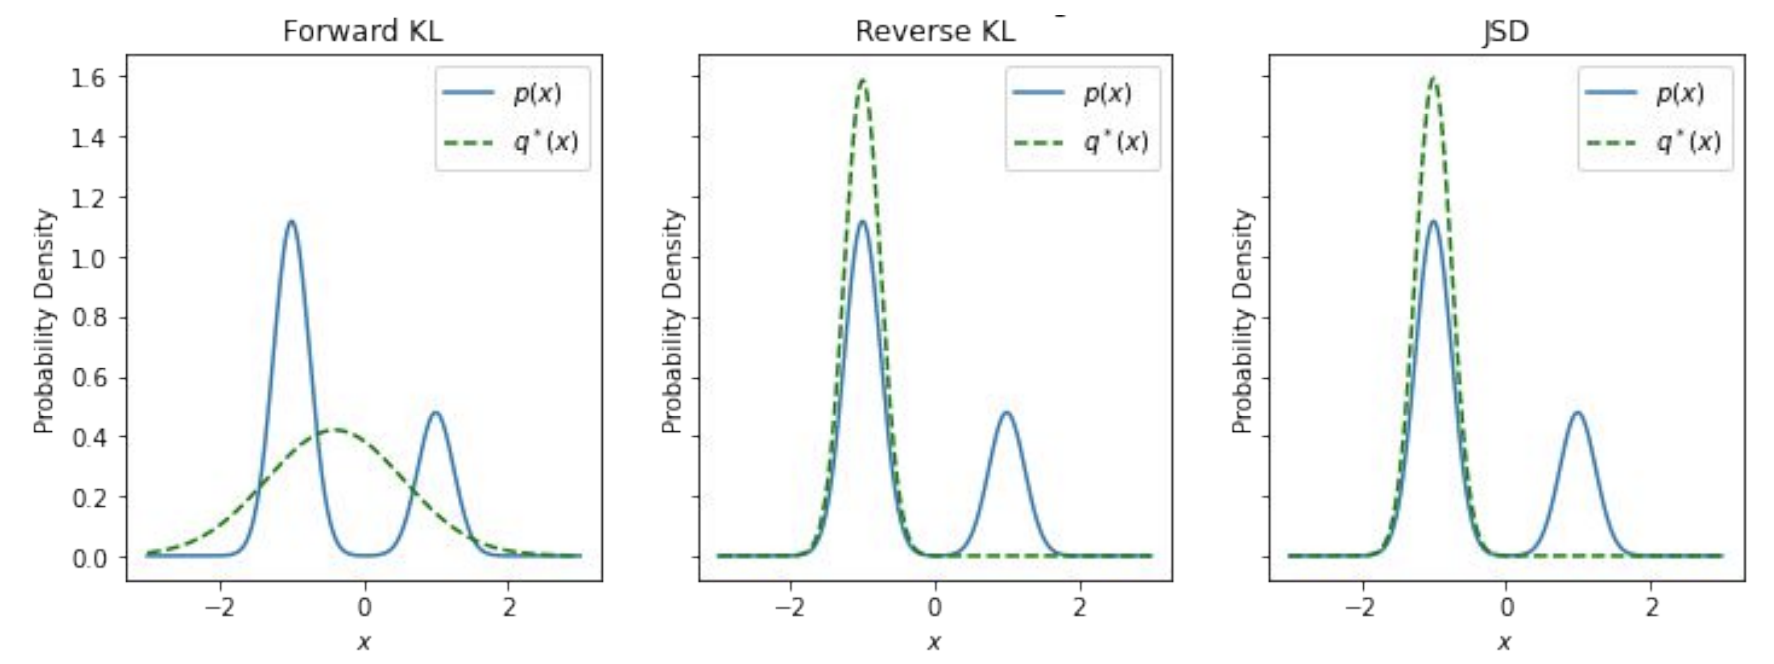
\includegraphics[width=0.7\linewidth]{figs/mode_collapse_2}
		\end{figure}
	\vspace{-0.3cm}
	\end{block}
	\myfootnotewithlink{https://sites.google.com/view/berkeley-cs294-158-sp20/home}{image credit: https://sites.google.com/view/berkeley-cs294-158-sp20/home}
\end{frame}
%=======
\begin{frame}{Vanila GAN results}
	\begin{figure}
		\centering
		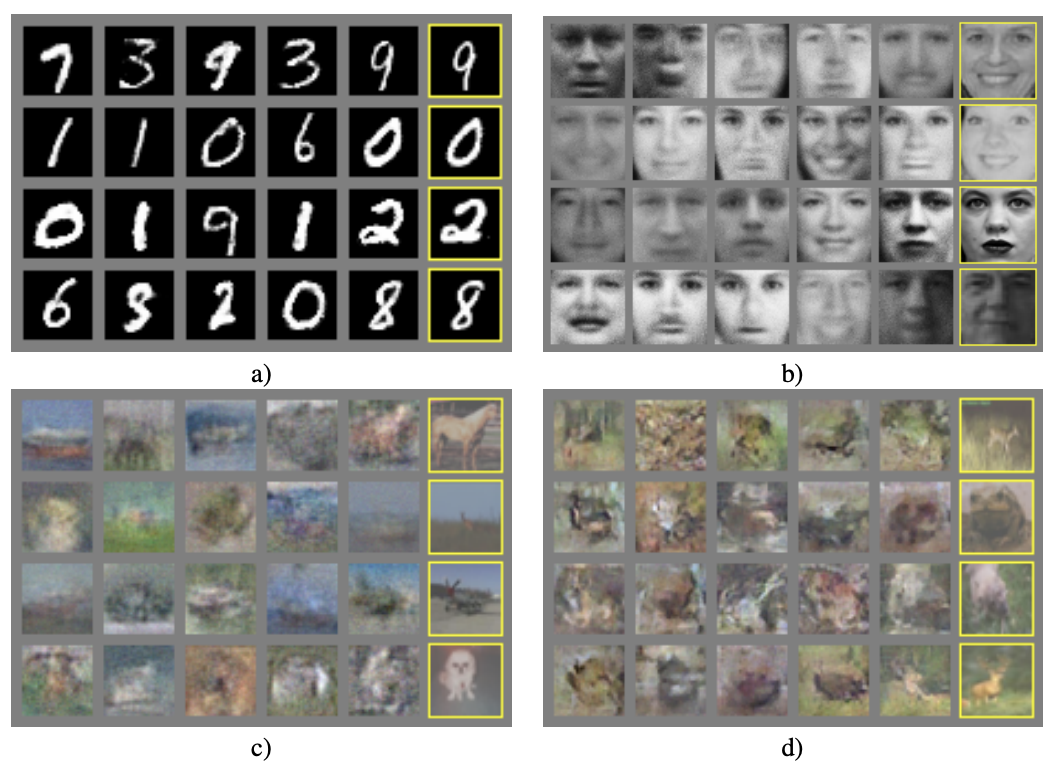
\includegraphics[width=0.95\linewidth]{figs/vanila_gan_results}
	\end{figure}
	\myfootnotewithlink{https://arxiv.org/abs/1406.2661}{Goodfellow I. J. et al. Generative Adversarial Networks, 2014}
\end{frame}
%=======
\begin{frame}{Deep Convolutional GAN}
	\begin{figure}
		\centering
		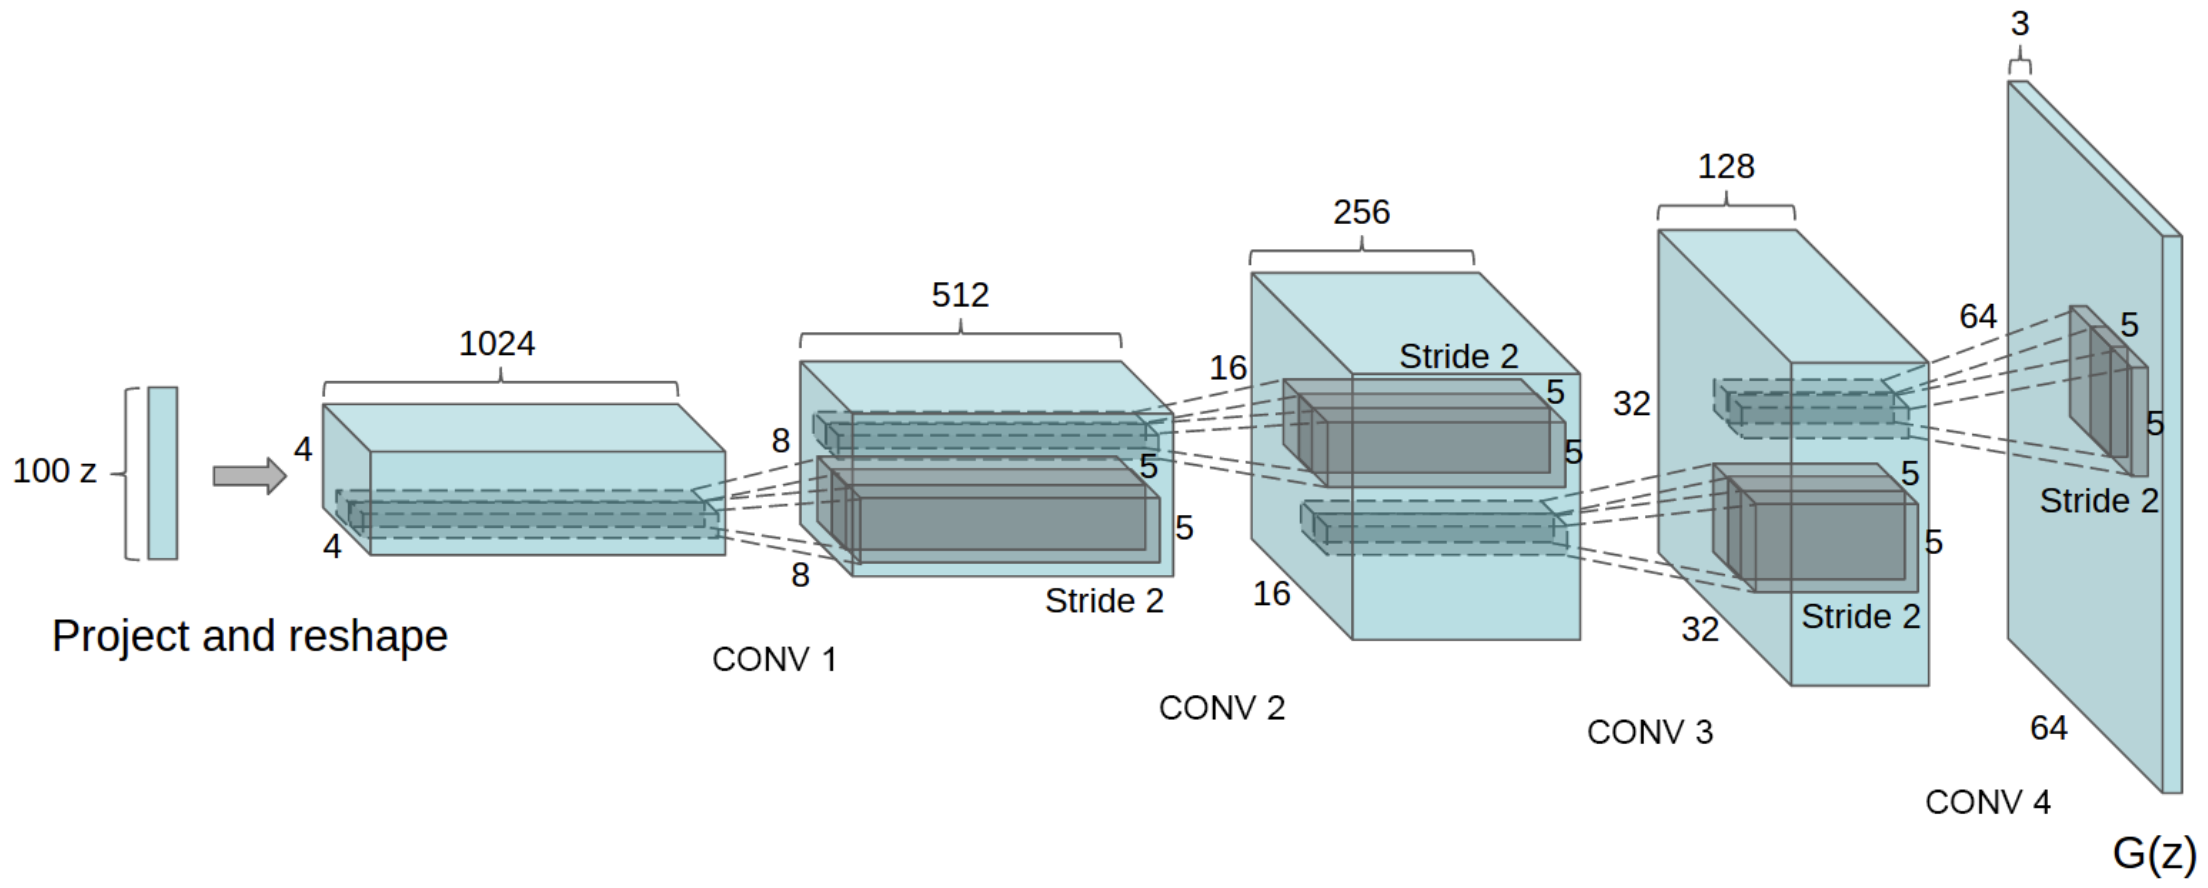
\includegraphics[width=0.8\linewidth]{figs/dcgan_1}
	\end{figure}
	\begin{itemize}
		\footnotesize
		\item  Mean-pooling instead of max-pooling.
		\item Transposed convolutions in the generator for upsampling.
		\item Downsample with strided convolutions and average pooling.
		\item ReLU for generator, Leaky-ReLU (0.2) for discriminator.
		\item Output nonlinearity: tanh for Generator, sigmoid for discriminator.
		\item Batch Normalization used to prevent mode collapse (not applied at the output of $G$ and input of $D$).
		\item Adam: small LR = 2e-4; small momentum: 0.5, batch-size: 128.
	\end{itemize}
	\myfootnotewithlink{https://arxiv.org/abs/1511.06434}{Radford A., Metz L., Chintala S. Unsupervised Representation Learning with Deep Convolutional Generative Adversarial Networks, 2015}
\end{frame}
%=======
\begin{frame}{Deep Convolutional GAN}
	\begin{block}{ImageNet samples}
		\begin{figure}
			\centering
			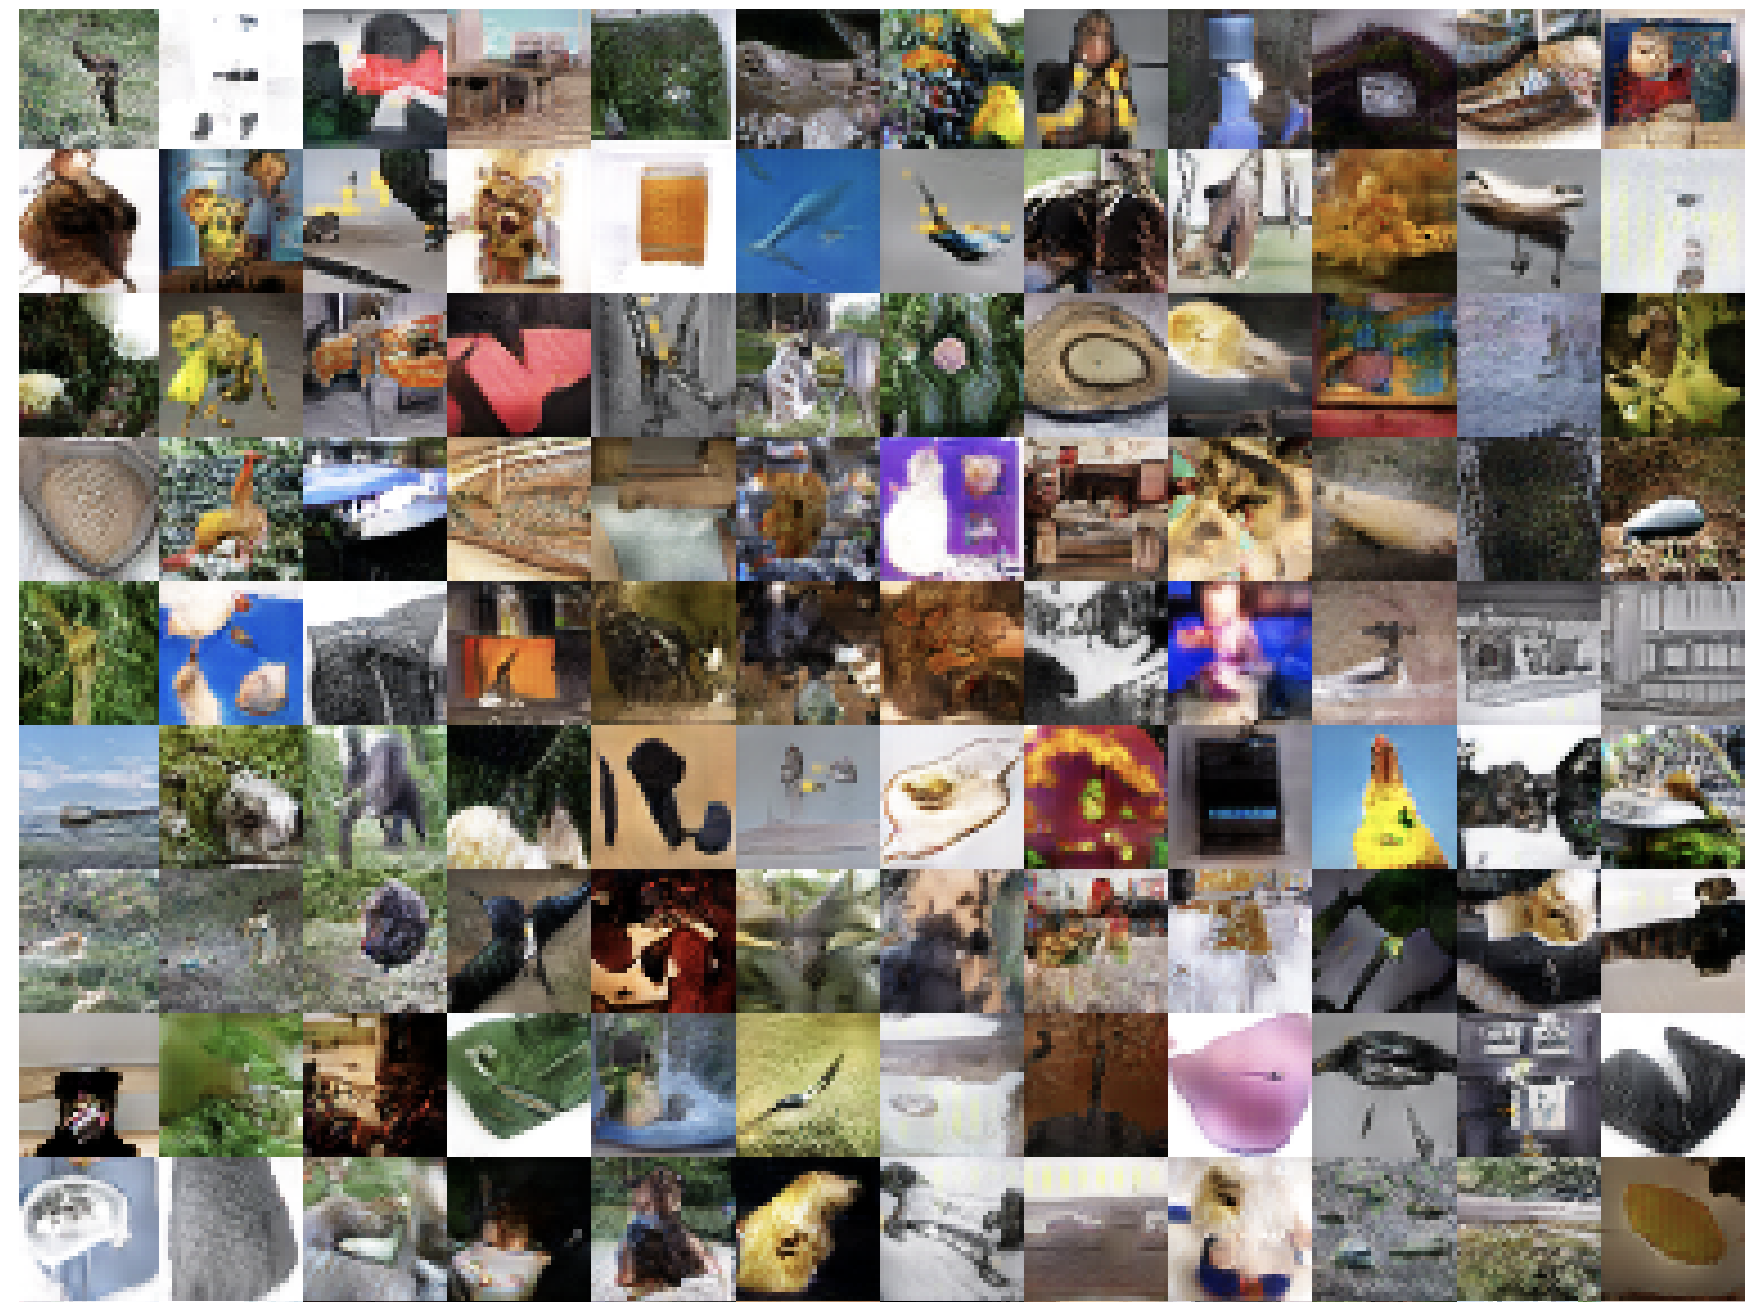
\includegraphics[width=0.8\linewidth]{figs/dcgan_results_1}
		\end{figure}
	\end{block}
	\myfootnotewithlink{https://arxiv.org/abs/1511.06434}{Radford A., Metz L., Chintala S. Unsupervised Representation Learning with Deep Convolutional Generative Adversarial Networks, 2015}
\end{frame}
%=======
\begin{frame}{Deep Convolutional GAN}
	\begin{block}{Smooth interpolations}
		\begin{figure}
			\centering
			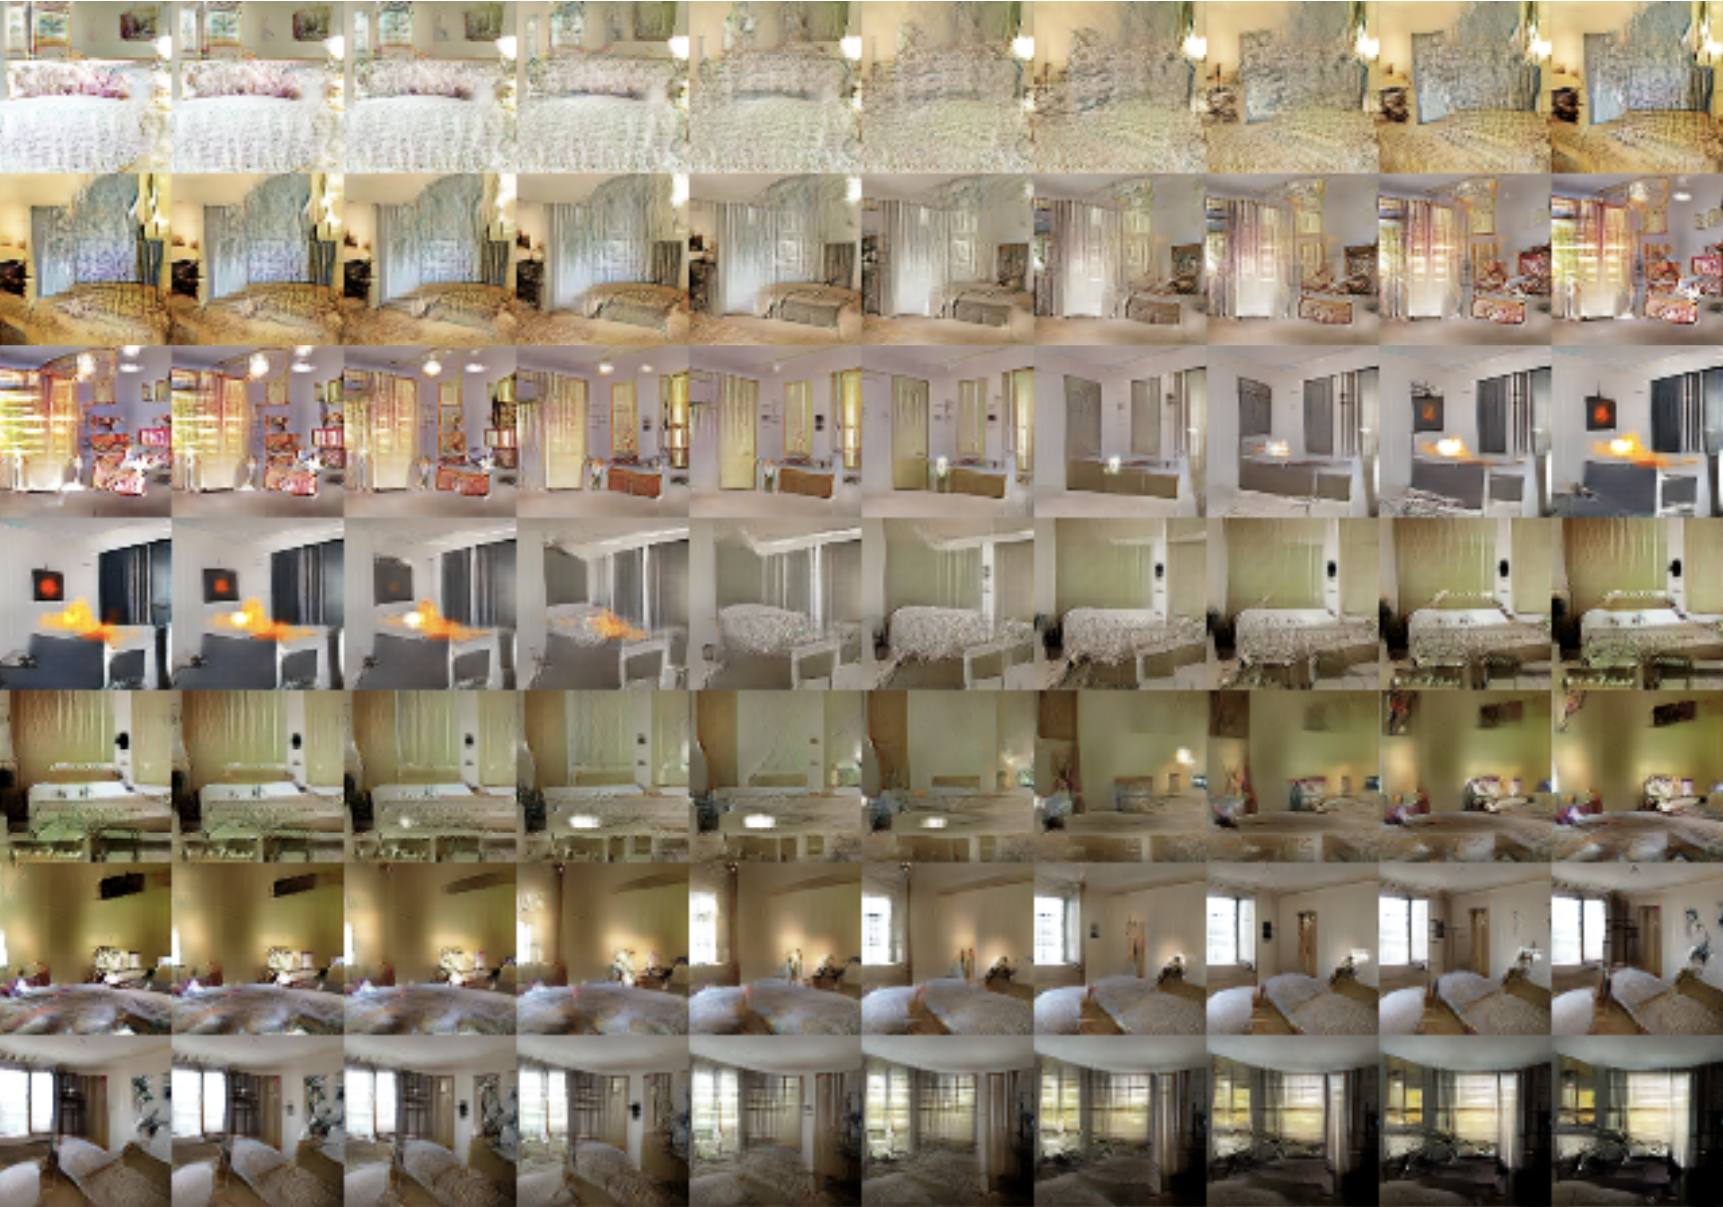
\includegraphics[width=0.8\linewidth]{figs/dcgan_results_2}
		\end{figure}
	\end{block}

	\myfootnotewithlink{https://arxiv.org/abs/1511.06434}{Radford A., Metz L., Chintala S. Unsupervised Representation Learning with Deep Convolutional Generative Adversarial Networks, 2015}
\end{frame}
%=======
\begin{frame}{Deep Convolutional GAN}
	\begin{block}{Vector arithmetic}
		\begin{figure}
			\centering
			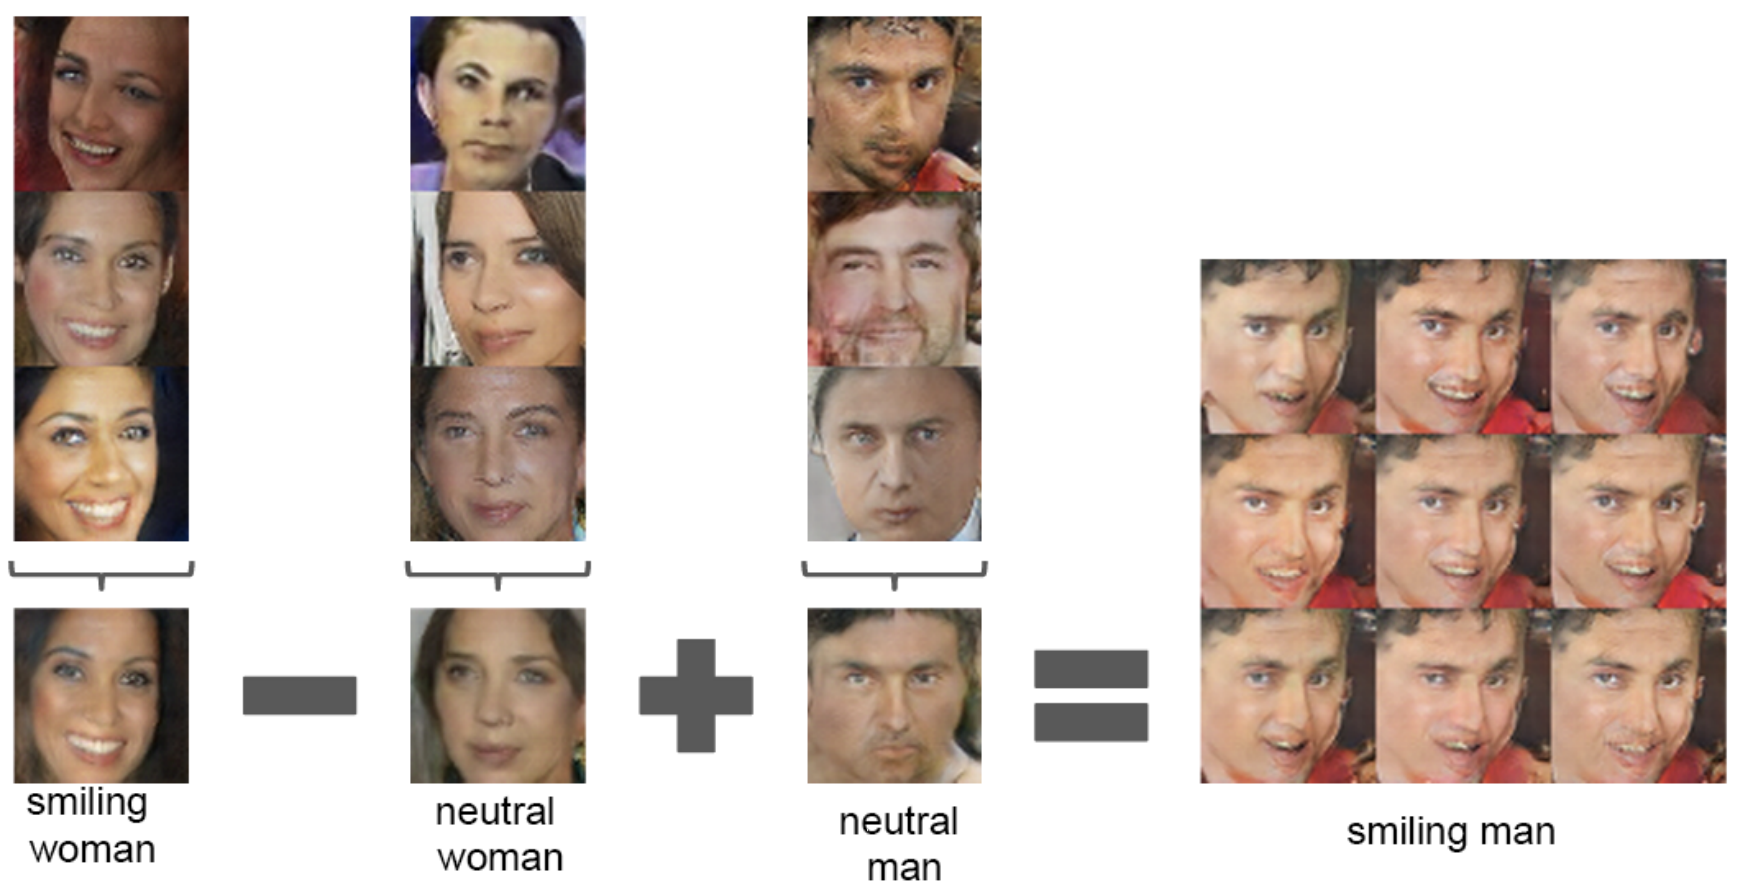
\includegraphics[width=1.0\linewidth]{figs/dcgan_results_3}
		\end{figure}
	\end{block}

	\myfootnotewithlink{https://arxiv.org/abs/1511.06434}{Radford A., Metz L., Chintala S. Unsupervised Representation Learning with Deep Convolutional Generative Adversarial Networks, 2015}
\end{frame}
%=======
\begin{frame}{Deep Convolutional GAN}
	\begin{block}{Mode collapse}
		\begin{figure}
			\centering
			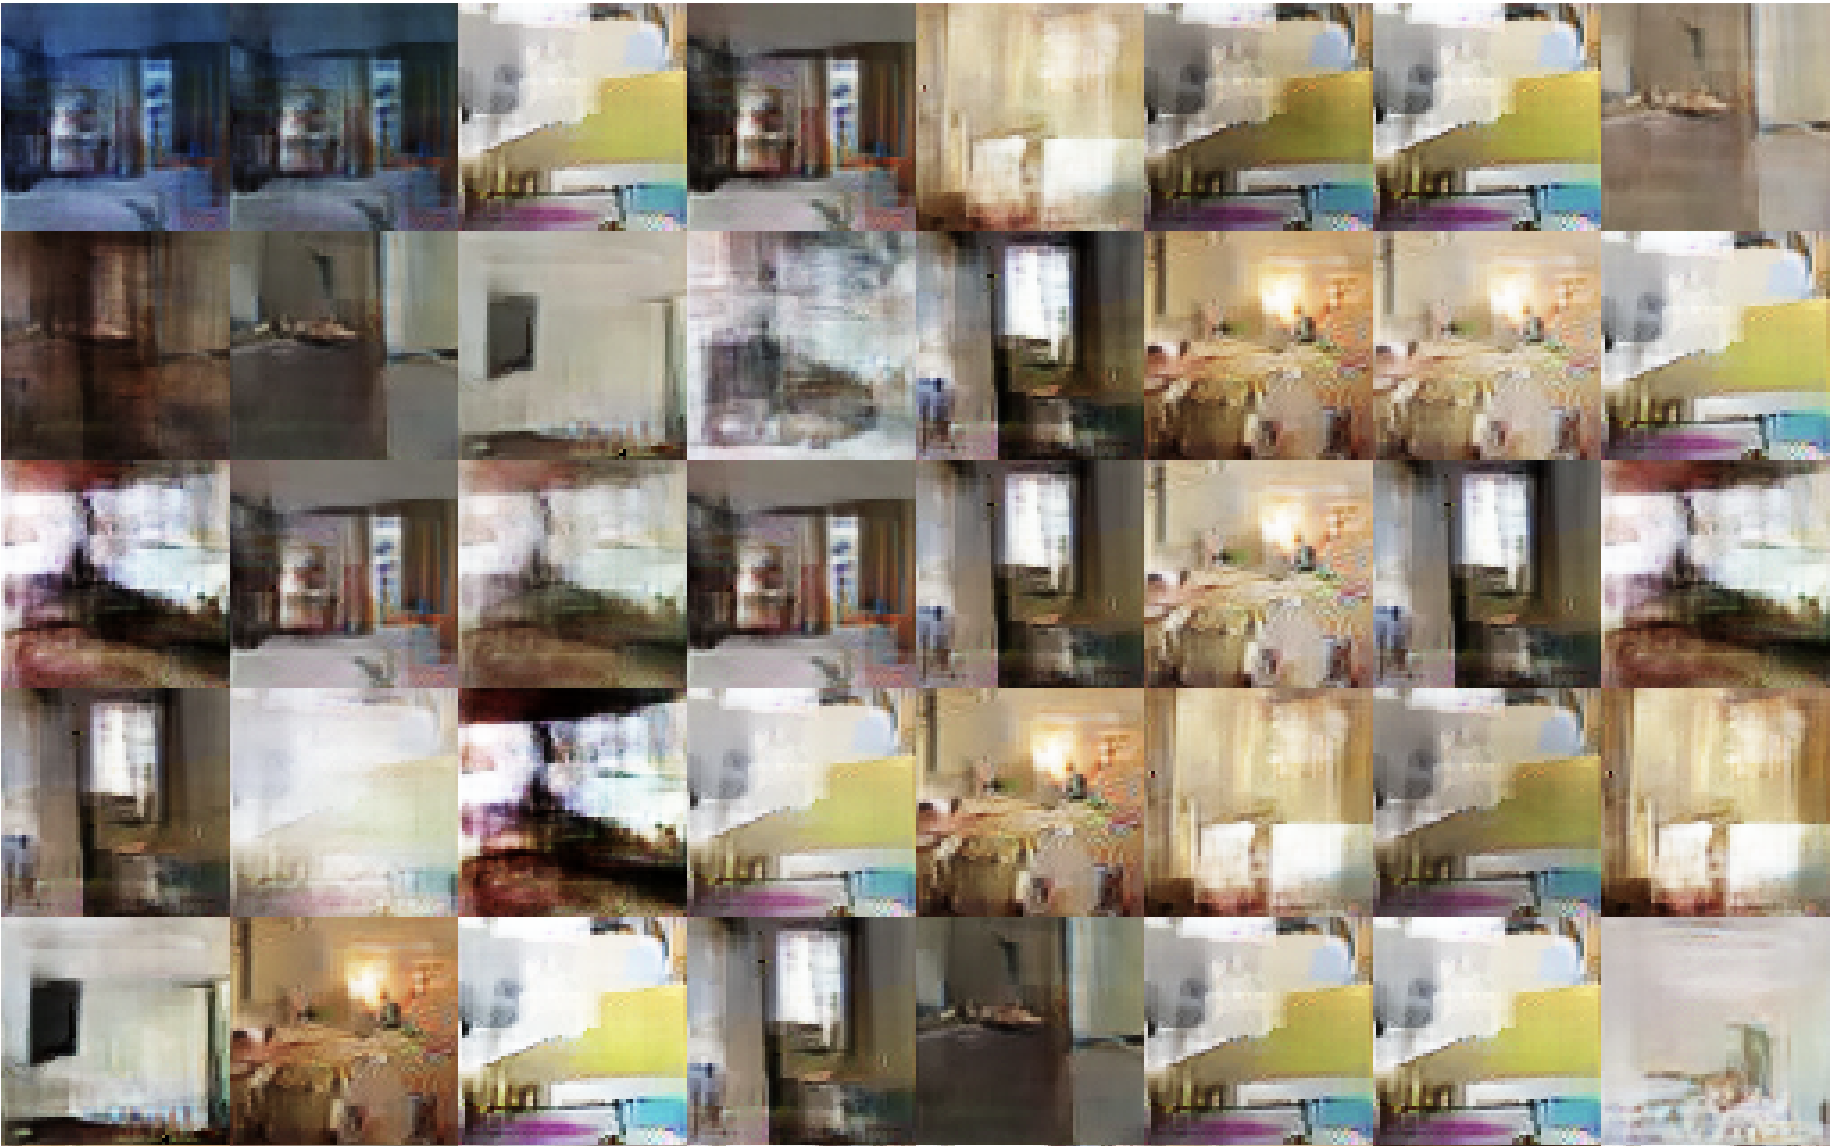
\includegraphics[width=0.95\linewidth]{figs/mode_collapse_4}
		\end{figure}
	\end{block}
	\myfootnotewithlink{https://arxiv.org/abs/1701.07875}{Arjovsky M., Chintala S., Bottou L. Wasserstein GAN, 2017}
\end{frame}
%=======
\begin{frame}{Improved techniques for training GANs}
	\begin{itemize}
		\item Feature matching
		\[
			\cL_G = \| \bbE_{\pi(\bx)} \mathbf{d}(\bx) - \bbE_{p(\bz)} \mathbf{d}(G(\bz)) \|_2^2
		\]
		Here $\mathbf{d}(\bx)$ -- intermediate layer of discriminator. Matching the learned discriminator statistics instead of the output of the discriminator. Helps to avoid the vanishing gradients for sufficiently good discriminator.
		\item Historical averaging adds extra loss term for generator and discriminator losses
		\vspace{-0.2cm}
		\[
		 \| \btheta - \frac{1}{T}\sum_{t=1}^T \btheta_t\|^2_2.
		\]
		Here $\btheta_t$ -- value of parameters at the previous step $t$. It allows to stabilize training procedure.
	\end{itemize}
	\myfootnotewithlink{https://arxiv.org/abs/1606.03498}{Salimans T. et al. Improved Techniques for Training GANs, 2016}
\end{frame}
%=======
\begin{frame}{Improved techniques for training GANs}
	\begin{itemize}
		\item One-sided label smoothing. Instead of using one-hot labels in classification, use $(1 - \alpha)$ for real data (the generated samples are not smoothed).
		\[
			D^*(\bx) = \frac{(1 - \alpha )\pi(\bx)}{\pi(\bx) + p(\bx | \btheta)}
		\]
		\item Virtual batch normalization. BatchNorm makes samples within minibatch are highly correlated.
		\begin{figure}
			\centering
			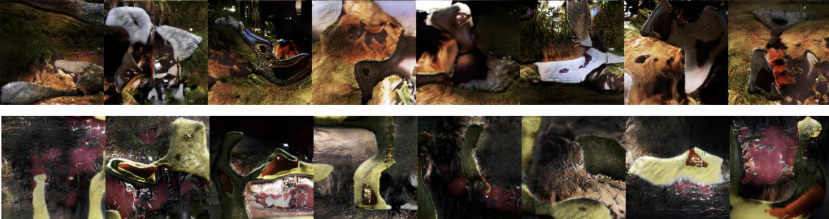
\includegraphics[width=0.6\linewidth]{figs/virtual_batch_norm}
		\end{figure}
	Use reference fixed batch to compute the normalization statistics. To avoid overfitting construct batch with the reference batch and the current sample. 
	\end{itemize}
	\myfootnotewithlink{https://arxiv.org/abs/1606.03498}{Salimans T. et al. Improved Techniques for Training GANs, 2016}
\end{frame}
%=======
\begin{frame}{Informal theoretical results}
	\begin{itemize}
		\footnotesize
		\item Since $\bz$ usually has lower dimensionality compared to $\bx$, manifold $G(\bz)$ has a measure 0 in $\bx$ space. Hence, support of $p(\bx | \btheta)$ lies on low-dimensional manifold.
		\item Distribution of real images $\pi(\bx)$ is also concentrated on a low dimensional manifold.
		\begin{figure}
			\centering
			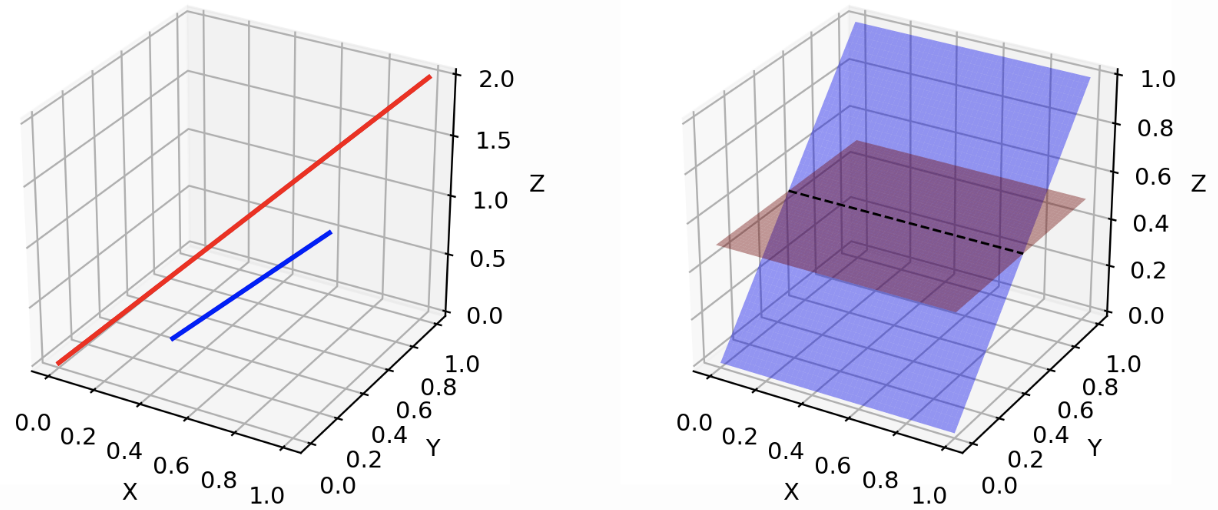
\includegraphics[width=0.5\linewidth]{figs/low_dim_manifold}
		\end{figure}
		\item If $\pi(\bx)$ and $p(\bx | \btheta)$ have disjoint supports, then there is a smooth optimal discrimator. We are not able to learn anything by backproping through it.
		\item For such low-dimensional disjoint manifolds
		\vspace{-0.1cm}
		\[
			KL(\pi || p) = KL(p || \pi) = \infty, \quad JSD(\pi || p) = \log 2
		\]
		\vspace{-0.7cm}
		\item Adding continuous noise to the inputs of the discriminator smoothes the distributions of the probability mass.
	\end{itemize}
	\myfootnote{\href{https://arxiv.org/abs/1904.08994}{Weng L. From GAN to WGAN, 2019} \\ 
	\href{https://arxiv.org/abs/1701.04862}{Arjovsky M., Bottou L. Towards Principled Methods for Training Generative Adversarial Networks, 2017}}
\end{frame}
%=======
\begin{frame}{Wasserstein distance (discrete)}
	Also called Earth Mover's distance.
	The minimum cost of moving and transforming a pile of dirt in the shape of one probability distribution to the shape of the other distribution.
	\begin{figure}
		\centering
		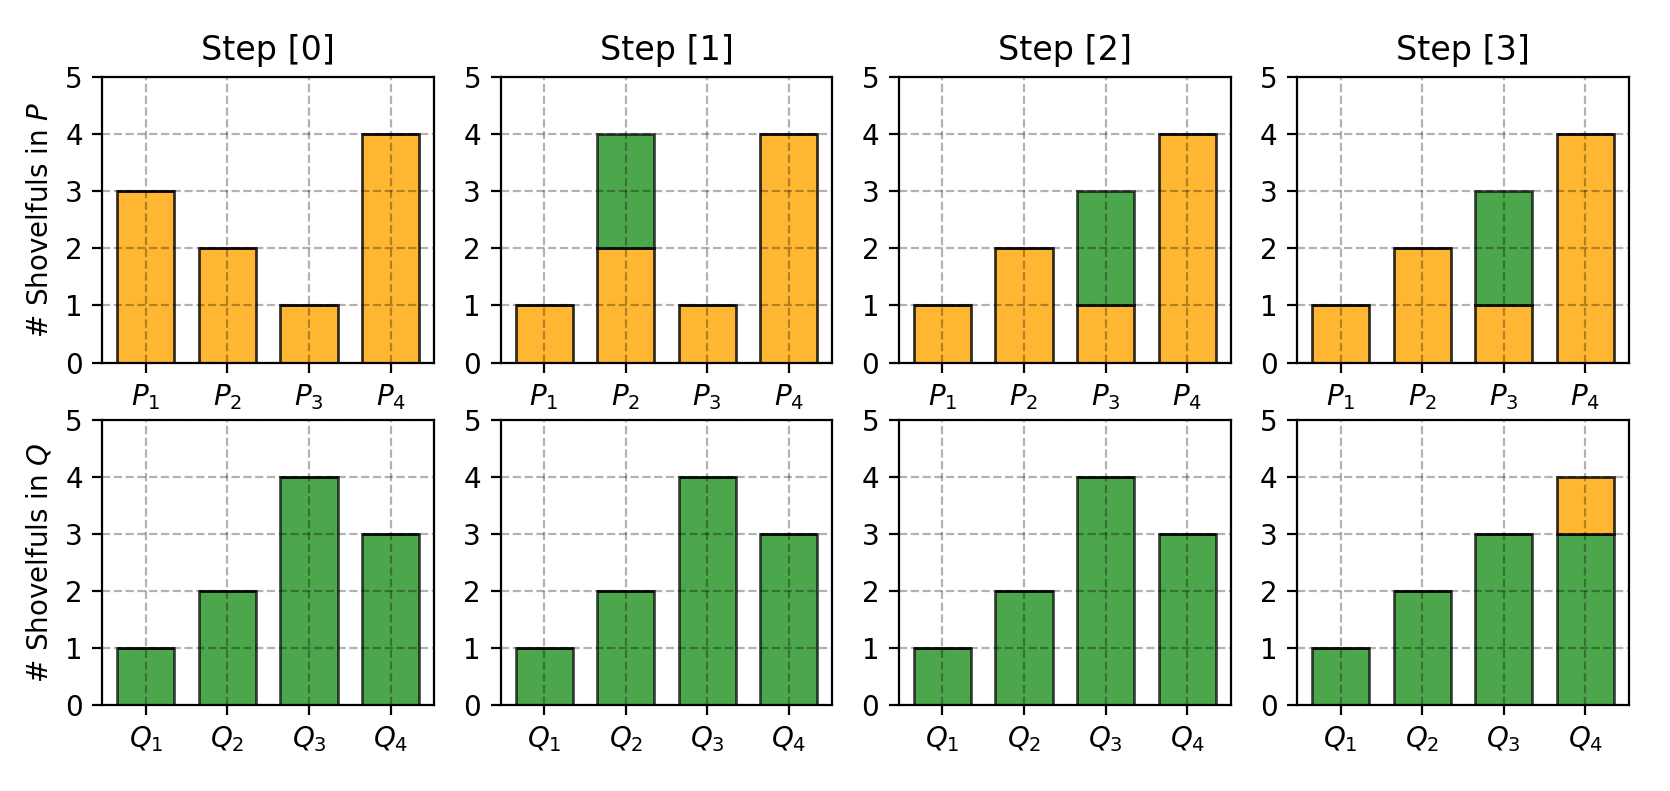
\includegraphics[width=.9\linewidth]{figs/EM_distance_discrete}
	\end{figure}
	\[
		W(P, Q) = 2 \text{(step 1)} + 2 \text{(step 2)} + 1 \text{(step 3)}  = 5
	\]
	\myfootnotewithlink{https://arxiv.org/abs/1904.08994}{Weng L. From GAN to WGAN, 2019} 
	
\end{frame}
%=======
\begin{frame}{Wasserstein distance}
	\[
		W(\pi, p) = \inf_{\gamma \in \prod(\pi, p)} \bbE_{(\bx, \by) \sim \gamma} \| \bx - \by \| =  \inf_{\gamma \in \prod(\pi, p)} \int \| \bx - \by \| \gamma (\bx, \by) d \bx d \by
	\]
	\begin{itemize}
		\item $\prod(\pi, p)$ -- the set of all joint distributions $\gamma (\bx, \by)$ with marginals $\pi$ and $p$ ($\int \gamma(\bx, \by) d \bx = p(\by)$, $\int \gamma(\bx, \by) d \by = \pi(\bx)$)
		\item $\gamma(\bx, \by)$ -- transportation plan (the amount of "dirt" that should be transported from point $\bx$ to point $\by$).
		\item $\gamma(\bx, \by)$ -- the amount, $\|\bx - \by \|$-- the distance.
	\end{itemize}
	For better understanding of transportation plan function $\gamma$, try to write down the plan for previous discrete case.
	\myfootnotewithlink{https://arxiv.org/abs/1701.07875}{Arjovsky M., Chintala S., Bottou L. Wasserstein GAN, 2017}
\end{frame}
%=======
\begin{frame}{Wasserstein distance vs KL vs JSD}
	
	\begin{minipage}[t]{0.48\columnwidth}
		\vspace{0.1cm}
		Consider 2d distributions
		\[
			\pi(x, y) = (0, U[0,1])
		\]	
		\[
			p(x, y | \theta) = (\theta, U[0, 1])
		\]
	\end{minipage}%
	\begin{minipage}[t]{0.52\columnwidth}
		\begin{figure}
			\centering
			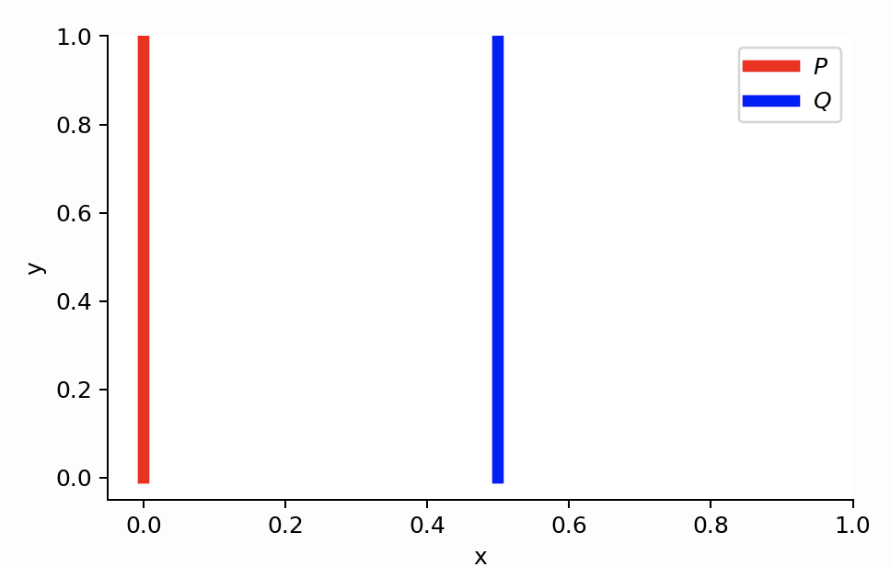
\includegraphics[width=0.8\linewidth]{figs/w_kl_jsd}
		\end{figure}
	\end{minipage}
	\begin{itemize}
		\footnotesize
		\item $\theta = 0$.
		Distributions are the same 
		\[
			KL(\pi || p) = KL(p || \pi) = JSD(p || \pi) = W(\pi, p) = 0
		\]
		\item $\theta \neq 0$
		\[
			KL(\pi || p) = \int_{U[0, 1]} 1 \log \frac{1}{0} d y = \infty = KL(p || \pi)
		\]
		\[
			JSD(\pi || p) = \frac{1}{2}\left( \int_{U[0, 1]}1 \log \frac{1}{1/2} dy + \int_{U[0, 1]}1 \log \frac{1}{1/2} dy \right) = \log 2
		\]
		\[
			W(\pi, p) = |\theta|
		\]
	\end{itemize}
	
	\myfootnote{\href{https://arxiv.org/abs/1904.08994}{Weng L. From GAN to WGAN, 2019} \\ 
	\href{https://arxiv.org/abs/1701.07875}{Arjovsky M., Chintala S., Bottou L. Wasserstein GAN, 2017}}
\end{frame}
%=======
\begin{frame}{Wasserstein distance vs KL vs JSD}
	\begin{block}{Theorem 1}
		Let $G(\bz, \btheta)$ be any feedforward neural network, and $p(\bz)$ a prior over $\bz$ such that $\bbE_{\bz \sim p(\bz)}
		\|\bz\| < \infty$. Then therefore $W(\pi, p)$ is continuous everywhere and differentiable almost everywhere.
	\end{block}
	\begin{block}{Theorem 2}
		Let $\pi$ be a distribution on a compact space $\cX$ and $\{p_t\}_{t=1}^\infty$ be a sequence of distributions on $\cX$. 
		\begin{align}
			KL(\pi || p_t) &\rightarrow 0 \, (\text{or }KL (p_t || \pi) \rightarrow 0) \\
			JSD(\pi || p_t) &\rightarrow 0 \\
			W(\pi || p_t) &\rightarrow 0
		\end{align}
		
		Then, considering limits as $t \rightarrow \infty$, (1) implies (2), (2) implies (3).
	\end{block}
	\myfootnotewithlink{https://arxiv.org/abs/1701.07875}{Arjovsky M., Chintala S., Bottou L. Wasserstein GAN, 2017}
\end{frame}
%=======
\begin{frame}{Summary}
	\begin{itemize}
	\item Majority of disentanglement learning models use heuristic objective or regularizers to achieve the goal.
	\end{itemize}
\end{frame}
%=======
\end{document} 